\documentclass[11pt,a4paper,oneside]{report}
\usepackage[T1]{fontenc}
\usepackage[utf8]{inputenc}
\usepackage{lmodern,microtype}
\usepackage[a4paper,margin=22mm,headheight=16pt]{geometry}
\usepackage{amsmath,amssymb,mathtools,bm}
\usepackage{graphicx,xcolor,booktabs,longtable,tabularx,array}
\usepackage{enumitem,fancyhdr,titlesec}
\usepackage[most]{tcolorbox}
\usepackage{tikz,pgfplots}
\usetikzlibrary{arrows.meta,positioning,calc}
\pgfplotsset{compat=1.18}
\usepackage{listings}
\usepackage[colorlinks=true,linkcolor=navy,citecolor=teal,urlcolor=teal,breaklinks=true]{hyperref}
\usepackage{bookmark}
\definecolor{navy}{HTML}{17334A}
\definecolor{teal}{HTML}{087F8C}
\definecolor{pale}{HTML}{EFF6F8}
\definecolor{amber}{HTML}{976016}
\definecolor{warm}{HTML}{FFF6E7}
\definecolor{grey}{HTML}{586675}
\hypersetup{pdftitle={Quantum Krylov and Sample-based Krylov Quantum Diagonalisation: A Study Companion},pdfauthor={A guided study companion},pdfsubject={Source-grounded companion to Ankush Kumar's October 8, 2026 manuscript}}
\setlength{\parindent}{0pt}
\setlength{\parskip}{6pt plus 1pt}
\setcounter{tocdepth}{0}
\bookmarksetup{depth=2}
\setcounter{secnumdepth}{2}
\setlist{nosep,leftmargin=1.5em,topsep=4pt}
\pagestyle{fancy}
\fancyhf{}
\fancyhead[L]{\small\sffamily\color{navy}Quantum Krylov \& Sample-based Diagonalisation}
\fancyhead[R]{\small\sffamily\color{grey}Study companion}
\fancyfoot[L]{\footnotesize\sffamily\color{grey}Theory \;\textbullet\; worked examples \;\textbullet\; manuscript analysis}
\fancyfoot[R]{\small\sffamily\thepage}
\renewcommand{\headrulewidth}{0.35pt}
\fancypagestyle{plain}{\fancyhf{}\fancyfoot[L]{\footnotesize\sffamily\color{grey}QKS + SKQD}\fancyfoot[R]{\small\sffamily\thepage}\renewcommand{\headrulewidth}{0pt}}
\titleformat{\chapter}[display]{\raggedright\hyphenpenalty=10000\normalfont\sffamily\bfseries\color{navy}}{\large\color{teal}CHAPTER \thechapter}{5pt}{\Huge}
\titlespacing*{\chapter}{0pt}{-12pt}{18pt}
\titleformat{\section}{\Large\sffamily\bfseries\color{navy}}{\thesection}{.65em}{}
\titleformat{\subsection}{\large\sffamily\bfseries\color{navy}}{\thesubsection}{.65em}{}
\newtcolorbox{idea}[1][Key idea]{enhanced,breakable,colback=pale,colframe=teal,boxrule=.6pt,arc=2mm,title=\sffamily\bfseries #1,fonttitle=\small,left=9pt,right=9pt,top=6pt,bottom=6pt}
\newtcolorbox{caution}[1][Important distinction]{enhanced,breakable,colback=warm,colframe=amber,boxrule=.6pt,arc=2mm,title=\sffamily\bfseries #1,fonttitle=\small,left=9pt,right=9pt,top=6pt,bottom=6pt}
\newtcolorbox{sourcebox}[1][What the manuscript reports]{enhanced,breakable,colback=white,colframe=grey,boxrule=.45pt,arc=1mm,title=\sffamily\bfseries #1,fonttitle=\small,colbacktitle=grey,left=9pt,right=9pt,top=6pt,bottom=6pt}
\newcommand{\ket}[1]{\lvert #1\rangle}
\newcommand{\bra}[1]{\langle #1\rvert}
\newcommand{\braket}[2]{\langle #1\vert #2\rangle}
\newcommand{\expect}[1]{\langle #1\rangle}
\newcommand{\norm}[1]{\left\lVert #1\right\rVert}
\newcommand{\abs}[1]{\left\lvert #1\right\rvert}
\newcommand{\Ht}{H_{\mathrm{tar}}}
\newcommand{\Hd}{H_{\mathrm{drive}}}
\newcommand{\HK}{H_{\mathcal K}}
\newcommand{\SK}{S_{\mathcal K}}
\newcommand{\HD}{H_{\mathcal D}}
\newcommand{\Dset}{\mathcal D}
\newcommand{\I}{\mathrm i}
\newcommand{\e}{\mathrm e}
\newcommand{\src}[1]{\par{\small\color{grey}\textit{Source status:} #1}\par}
\newcommand{\checkpoint}[1]{\begin{idea}[Check your understanding]#1\end{idea}}
\newcolumntype{Y}{>{\raggedright\arraybackslash}X}
\lstset{basicstyle=\ttfamily\footnotesize,breaklines=true,columns=fullflexible,keepspaces=true,frame=single,rulecolor=\color{grey!35},backgroundcolor=\color{pale!45},showstringspaces=false,tabsize=4}
\pgfplotsset{every axis/.append style={width=.91\linewidth,height=6.5cm,grid=major,major grid style={gray!20},tick label style={font=\small},label style={font=\small},legend style={font=\small,draw=none},line width=1pt}}
\begin{document}
\begin{titlepage}
\pagecolor{navy}\color{white}
\vspace*{14mm}
{\sffamily\large A GUIDED COURSE + RESEARCH COMPANION\par}
\vspace{15mm}
{\sffamily\bfseries\fontsize{35}{40}\selectfont Quantum Krylov\par Subspace Methods\par}
\vspace{8mm}
{\sffamily\fontsize{25}{30}\selectfont Sample-based Krylov\par Quantum Diagonalisation\par}
\vspace{14mm}
{\Large From eigenvalue problems to Ankush's\par trapped-ion chemistry workflow\par}
\vspace{14mm}
\begin{tikzpicture}
\draw[white,line width=1.2pt] (0,0)--(14,0);
\end{tikzpicture}\par
\vspace{5mm}
{\large Intuition, derivations, and numerical stability.\par Chemistry, worked examples, and research directions.\par}
\vfill
{\sffamily\large A guided study companion\par}
\vspace{4mm}
{\normalsize Manuscript studied: Ankush Kumar, 8 October 2026.\par Companion expanded: 9 October 2026.\par}
\vspace{8mm}
{\small Original teaching simulations are clearly separated from reported hardware results.\par}
\end{titlepage}
\nopagecolor\color{black}
\pagenumbering{roman}
\chapter*{How to use this course}
\addcontentsline{toc}{chapter}{How to use this course}
This expanded edition includes a step-by-step molecule-to-qubit derivation (Chapter 1) before taking you beyond recognising the formula $Hc=ESc$. By the end, you should be able to explain what is prepared on the quantum processor, what is measured, what is computed classically, why the answer can improve, and which assumptions might fail.

The starting point is the uploaded manuscript by \textbf{Ankush Kumar}, \textit{Scalable Non-Iterative Quantum Krylov Subspace Chemistry on Trapped-Ion Processors: Solving Polyatomic and Aromatic Ground States within Chemical Precision on Quantinuum H-Series}, dated 8 October 2026 \cite{kumar}. The accompanying pasted explanation and the added molecule-to-qubit walkthrough are used as learning scaffolds, not as independent evidence \cite{pasted}.

\begin{idea}[The one distinction to keep in view]
Conventional quantum Krylov diagonalisation uses \emph{time-evolved states as basis vectors}. Sample-based Krylov diagonalisation uses those states to \emph{discover basis configurations}, then diagonalises the target Hamiltonian in the configuration space. These are generally different subspaces.
\end{idea}

\section*{Four passes through the material}
\textbf{Pass 1: see the mechanism.} Read Chapter 1 from the coordinate Hamiltonian to the Pauli mapping, then Chapters 2--3 and the two-state example in Chapter 4. You should be able to derive the projected eigenproblem and explain why real-time evolution alone does not cool a state.

\textbf{Pass 2: understand the change to sampling.} Read Chapters 5--7. Explain $S=I$, the distinction between the target and driving Hamiltonians, and the limitations of support discovery.

\textbf{Pass 3: read Ankush's work operationally.} Read Chapters 8--10 alongside the manuscript. Reconstruct its water workflow, classify every number as reported or derived, and identify the missing inputs for replication.

\textbf{Pass 4: become a contributor.} Run the laboratory, solve the exercises, and use Chapters 11--12 to design controlled extensions. Do not skip classical-only baselines.

\section*{What the source labels mean}
\begin{tabularx}{\linewidth}{@{}p{30mm}Y@{}}
\toprule
Label & Interpretation\\\midrule
\textbf{[M]} & The uploaded manuscript. Section/page/equation references refer to its printed pages. Its hardware outcomes are \emph{reported results}, not independently verified here.\\
\textbf{[P]} & The uploaded pasted explanation. Useful structure, but not a primary research source.\\
\textbf{[K], [S],\ldots} & External primary literature or official documentation, cited to distinguish established methods from manuscript-specific choices.\\
\textbf{Derivation / lab} & Calculations developed in this companion, with assumptions stated. Numerical examples are small classical simulations.\\
\textbf{Clarification needed} & Information not supplied, or a claim whose interpretation requires code, data, or additional assumptions.\\\bottomrule
\end{tabularx}

\section*{What these materials cannot reconstruct from the uploads alone}
The uploads do not contain the full molecular integrals, orbital coefficients, tapered Pauli lists, symmetry generators and sectors, native circuits, raw count files, expansion thresholds, exact benchmark energies, or execution logs. Consequently, the included program \textbf{does not reproduce the water or fluorine hardware energies}. It reproduces independently specified teaching examples and provides reusable numerical building blocks.

\begin{caution}[Reading critically is not dismissing the work]
A useful hardware workflow can be valuable even when a manuscript overstates its guarantees or leaves out implementation details. We preserve the reported procedure, then explicitly distinguish it from what follows mathematically. A result agreeing with a small active-space reference is not, by itself, evidence of quantum advantage or of full-molecule chemical accuracy.
\end{caution}

\section*{Deliverables and execution}
The accompanying PowerPoint follows the same learning progression and contains speaker notes. The source of this PDF is a single self-contained \texttt{.tex} file: its teaching plots use embedded coordinates, and its bibliography is included. Compile twice with \texttt{pdflatex}, or use \texttt{latexmk -pdf}. The laboratory requires only NumPy and SciPy; the figure script additionally requires Matplotlib.

\tableofcontents
\clearpage
\chapter*{Notation and the three spaces}
\addcontentsline{toc}{chapter}{Notation and the three spaces}
\begin{tabularx}{\linewidth}{@{}p{26mm}Y@{}}
\toprule Symbol & Meaning in this companion\\\midrule
$n$ & Qubits in the representation currently being used.\\
$m$ & Spatial orbitals in an active space; there are $2m$ spin orbitals.\\
$N_\alpha,N_\beta$ & Active electrons of each spin in a fixed spin-projection sector.\\
$\Ht$ & Target Hamiltonian after the declared active-space choice and any exact sector reduction; all its retained physical interactions are used in final projection.\\
$\Hd$ & Hamiltonian used to generate sample-producing states; it need not equal $\Ht$.\\
$\ket r$ & Normalised reference state, often a Hartree--Fock determinant before tapering.\\
$K$ & Number of time points / coherent Krylov vectors, not number of Pauli terms.\\
$L_{\rm drive}$ & Number of selected off-diagonal drive terms; [M] often calls this $K$.\\
$D$ & Number of distinct selected basis configurations.\\
$\Phi$ & Matrix with coherent Krylov states as columns.\\
$\HK,\SK$ & Projected target Hamiltonian and overlap/Gram matrix in the coherent basis.\\
$B_\Dset$ & Isometry whose columns are distinct selected orthonormal configurations.\\
$\HD$ & $B_\Dset^\dagger\Ht B_\Dset$, the sampled-space Hamiltonian.\\
$E_0,\Delta$ & Ground energy and spectral gap of the \emph{declared target sector}.\\
$N_k$ & Number of circuit executions (shots) allocated to time $t_k$.\\
$\tau_S,\eta_{\rm prune}$;\newline $\eta_E,\epsilon_{\rm expand}$ & Distinct thresholds for Gram truncation, term pruning, energetic filtering, and connected expansion.\\\bottomrule
\end{tabularx}

There are three different dimensions: the full active Hilbert space, the coherent span of at most $K$ states, and the sampled coordinate space of $D$ states. \textbf{Never use one dimension as a proxy for another.}

We set $\hbar=1$. When Hamiltonian coefficients are in Hartree, a time in $\e^{-\I Ht}$ is in inverse Hartree (atomic units of time). Circuit libraries may parameterise rotations in radians or half-turns; conversion is an implementation input, not a typographical detail.

For worked bitstring examples, displayed strings are $b_{n-1}\cdots b_0$. Integer bit $p$ labels qubit/orbital $p$. Pauli labels use the same left-to-right ordering. These conventions are explicitly implemented in the laboratory.

\clearpage\pagenumbering{arabic}
\chapter{Molecular energy as an eigenvalue problem}\label{ch:chem}
\src{Background derivations; chemistry setting from [M], Sections 1 and 3.1. The counting clarification below is explicit, not a silent replacement of [M], Eq. (2).}

\section{What is the answer we are trying to compute?}
For fixed nuclear positions, the electronic problem is
\begin{equation}
\Ht\ket{E_j}=E_j\ket{E_j},\qquad E_0\le E_1\le\cdots.
\end{equation}
The ground energy is the smallest Rayleigh quotient,
\begin{equation}\label{eq:rayleigh}
E_0=\min_{\ket\psi\ne0}\frac{\bra\psi\Ht\ket\psi}{\braket\psi\psi}.
\end{equation}
A chemistry calculation first defines an approximation to the physical problem: nuclear geometry, basis set, orbitals, frozen orbitals, active electrons, and symmetry sector. An accurate eigenvalue of the resulting matrix is only accurate \emph{for that chosen model}.

The manuscript uses a $1.6$ mHa accuracy threshold, where $1$ mHa $=10^{-3}$ Ha \cite{kumar}. Record the reference against which this error is measured. Comparing against CASCI in a six-orbital space is different from comparing against all-electron FCI in the full basis, and both differ from experiment.


\section{Start with a real molecule: the water example}
\src{Expanded teaching derivation adapted from the additional explanation provided in the conversation; the underlying electronic Hamiltonian is standard quantum-chemistry background, not a separate claim in [M].}

A water molecule contains three nuclei (one oxygen, two hydrogens) and ten electrons in a neutral, all-electron description. The nuclei have positions $\mathbf R_A$ and charges $Z_A$, and the electrons have positions $\mathbf r_i$. Under the \emph{Born--Oppenheimer approximation}, we hold the nuclei at a specified geometry while solving the electronic problem. The corresponding nonrelativistic, clamped-nuclei Hamiltonian in atomic units is
\begin{equation}\label{eq:coordinateH}
\boxed{\displaystyle
H_{\rm mol}=-\sum_{i=1}^{N}\frac{\nabla_i^2}{2}
-\sum_{i=1}^{N}\sum_{A=1}^{N_{\rm nuc}}\frac{Z_A}{|\mathbf r_i-\mathbf R_A|}
+\sum_{1\le i<j\le N}\frac1{|\mathbf r_i-\mathbf r_j|}
+E_{\rm nuc}.}
\end{equation}
Here $E_{\rm nuc}=\sum_{A<B}Z_AZ_B/|\mathbf R_A-\mathbf R_B|$ is constant when the nuclear geometry is held fixed.

\begin{center}
\small
\begin{tabularx}{\linewidth}{@{}p{58mm}Y@{}}
\toprule
Term & What it means physically\\\midrule
$-\sum_i\nabla_i^2/2$ & Electronic kinetic energy: electrons can move.\\
$-\sum_{i,A}Z_A/|\mathbf r_i-\mathbf R_A|$ & Electron--nucleus Coulomb attraction.\\
$\sum_{i<j}1/|\mathbf r_i-\mathbf r_j|$ & Electron--electron Coulomb repulsion.\\
$E_{\rm nuc}$ & Repulsion of nuclei at the chosen fixed geometry.\\\bottomrule
\end{tabularx}
\end{center}

An eigenvalue $E$ of this Hamiltonian, with the constant $E_{\rm nuc}$ included, is an electronic-potential-energy value at that nuclear geometry. If a reference Hamiltonian omits this scalar or uses frozen-core offsets, those constants must be put back before comparing absolute molecular energies. Solving the problem at several geometries gives a \emph{potential-energy surface}.

\begin{idea}[Why this matters for Krylov and SKQD]
The continuous wavefunction lives in an enormous function space. QKS and SKQD do not start by inserting the differential operator $-\nabla^2/2$ directly into gates. They first work with a \emph{finite, explicitly chosen} electronic Hamiltonian, which is then encoded as qubit operations.
\end{idea}

\section{A finite orbital basis turns the wavefunction into algebra}
Choose a finite collection of $M$ orthonormal \emph{spin orbitals} $\chi_p(x)$, with $x=(\mathbf r,\sigma)$ containing spatial position and spin. The orbital basis (for example, one generated using STO-3G) specifies which one-particle shapes we allow. It also determines the molecular integrals used below.

\begin{enumerate}[label=\textbf{\arabic*.}]
\item \textbf{Basis set:} approximate the continuous electronic wavefunction using finitely many orbital functions. The basis choice introduces a controllable but generally nonzero model error.
\item \textbf{Hartree--Fock reference:} solve a mean-field problem to get orbitals and a convenient initial determinant $\ket{\Phi_{\rm HF}}$.
\item \textbf{Active-space choice:} if the full basis is too large, retain selected active orbitals and electrons. A CAS$(N_e e,m o)$ calculation means $N_e$ active electrons in $m$ spatial orbitals, or $2m$ spin orbitals before further reductions.
\item \textbf{Symmetry sector:} particle number, spin labels where conserved, and parity symmetries restrict which eigenvalue is physically relevant.
\end{enumerate}

\begin{caution}[Three different approximations]
Fixing a nuclear geometry is the clamped-nuclei modelling step; a finite basis and an active space restrict the \emph{target Hamiltonian}; exact tapering (performed in a correct sector) merely changes how that target is \emph{represented}. None of these should be conflated with error from QKS or SKQD itself.
\end{caution}

\section{From orbitals to determinants}
An orbital is a one-electron function. A spin orbital includes the spin label. A Slater determinant is an antisymmetric many-electron basis state described by which spin orbitals are occupied. In an orthonormal orbital basis, distinct occupation patterns give orthonormal determinants.

For $m$ spatial orbitals there are $m$ spin-up and $m$ spin-down orbitals. If $N_\alpha$ and $N_\beta$ are fixed, then
\begin{equation}\label{eq:count}
D_{N_\alpha,N_\beta}=\binom{m}{N_\alpha}\binom{m}{N_\beta}.
\end{equation}
If only the total particle number $N$ is fixed, the count is $\binom{2m}{N}$. With no particle-number restriction, the Fock-space dimension is $2^{2m}$.

\begin{caution}[Counting clarification: manuscript Eq. (2)]
{[M]} describes $M$ as the number of spatial orbitals but prints $\binom{2M}{N_\alpha}\binom{2M}{N_\beta}$. With that definition of $M$, each spin species has $M$, not $2M$, available orbitals. Equation~\eqref{eq:count} is the correct fixed-spin-sector count. Binomial growth is exponential at fixed filling; ``factorial scaling'' is not the most precise asymptotic description.
\end{caution}

For CAS$(8e,6o)$ and $N_\alpha=N_\beta=4$, the count is $15^2=225$. For CAS$(10e,6o)$ with $N_\alpha=N_\beta=5$, it is $6^2=36$. For CAS$(6e,6o)$ with balanced spins it is $20^2=400$. These small dimensions will matter when evaluating the manuscript's benchmarks.

\section{Hartree--Fock, CI, CASCI, and CASSCF}
\textbf{Hartree--Fock (HF)} optimises a single determinant. It supplies orbitals and a reference but cannot describe an arbitrary correlated state. \textbf{Configuration interaction (CI)} uses a linear combination of determinants. \textbf{FCI} includes every determinant in the declared orbital and electron space. \textbf{CASCI} performs full CI within a selected active orbital space while keeping the orbitals fixed. \textbf{CASSCF} additionally optimises orbitals.

A CAS label specifies active electrons and spatial orbitals; it does not specify which orbitals were selected or how they were obtained. Two CAS$(6e,6o)$ calculations can represent different Hamiltonians. Reproduction requires the actual orbitals/integrals and energy offsets, not merely the CAS label.

\begin{idea}[Active-space reduction versus tapering]
Choosing an active space usually changes the model relative to the full electronic problem. Exact symmetry tapering changes the representation of a specified sector \emph{without changing that sector's spectrum}. These reductions must not be assigned the same error interpretation.
\end{idea}


\section{Second quantisation: occupation instead of electron coordinates}
In first-quantised language we describe an antisymmetric wavefunction of $N$ labelled coordinate slots. In \emph{second quantisation}, we instead describe occupation of spin orbitals, using $a_p^\dagger$ to create an electron in orbital $p$ and $a_p$ to remove one. The \emph{Fock vacuum} $\ket{\mathrm{vac}}$ contains no electrons. A properly ordered $N$-electron Slater determinant is
\begin{equation}
\ket{D_{p_1\cdots p_N}}=a_{p_1}^\dagger a_{p_2}^\dagger\cdots a_{p_N}^\dagger\ket{\mathrm{vac}},
\qquad p_1<p_2<\cdots<p_N,
\end{equation}
up to the specified global ordering convention. The Pauli principle is enforced by the \emph{fermionic anticommutation relations}
\begin{equation}\label{eq:anticommutators}
\{a_p,a_q^\dagger\}=\delta_{pq}I,\qquad
\{a_p,a_q\}=\{a_p^\dagger,a_q^\dagger\}=0.
\end{equation}
In particular, $(a_p^\dagger)^2=0$: you cannot create two electrons in the same spin orbital.

A convenient spin-orbital integral convention is
\begin{align}
 h_{pq}&=\int\!dx\,\chi_p^*(x)
 \left(-\tfrac12\nabla^2-\sum_A\frac{Z_A}{|\mathbf r-\mathbf R_A|}\right)\chi_q(x),\\
 g_{pqrs}&=\iint\!dx\,dy\,\chi_p^*(x)\chi_q^*(y)
 \frac{\chi_r(x)\chi_s(y)}{|\mathbf r_x-\mathbf r_y|}.
\end{align}
With $g_{pqrs}=\langle pq|rs\rangle$ defined \emph{exactly} in that index order, the finite-basis Hamiltonian takes the form
\begin{equation}\label{eq:fermionH}
\boxed{\displaystyle H_{\rm ferm}=E_{\rm const}
+\sum_{pq}h_{pq}a_p^\dagger a_q
+\frac12\sum_{pqrs}g_{pqrs}a_p^\dagger a_q^\dagger a_s a_r.}
\end{equation}
The first sum contains kinetic energy and electron--nucleus attraction. The second contains pairwise electron repulsion. For an all-electron active basis, $E_{\rm const}=E_{\rm nuc}$; when cores are frozen, there are additional one-body adjustments and a scalar core-energy offset. Equivalent textbook formulas may instead use antisymmetrised integrals with $1/4$; the prefactor and index order must agree.

\begin{idea}[How a matrix appears]
The entries $h_{pq}$ and $g_{pqrs}$ are \emph{ordinary numbers} obtained by classical integration and orbital calculations. Creation and annihilation operators tell us \emph{which occupation basis states are coupled}. Thus the differential-operator problem of Eq.~\eqref{eq:coordinateH} becomes a finite Hermitian eigenvalue problem, even before choosing a quantum computer.
\end{idea}

\subsection{What is an occupation bitstring?}
Each spin orbital has occupation $n_p\in\{0,1\}$, so a register of four spin orbitals can encode two occupied orbitals by a pattern with two ones. \textbf{Bit-order conventions differ across textbooks and software.} This companion writes displayed strings as $b_{n-1}\cdots b_1b_0$ (orbital zero on the \emph{right}), so the occupation $n_0=n_1=1$, $n_2=n_3=0$ is written $\ket{0011}$. If you instead list orbital zero on the left, the same occupation is written $\ket{1100}$. The underlying state is identical once the convention is fixed.

\section{Qubit mapping: fermions become Pauli strings}
A quantum processor controls qubit operators, not abstract fermionic creation and annihilation operators. The \emph{Jordan--Wigner transformation} maps orbital $p$ to qubit $p$ and uses a string of $Z$ operators to preserve fermionic signs:
\begin{align}\label{eq:JW}
 a_p^\dagger&=\left(\prod_{j=0}^{p-1}Z_j\right)\frac{X_p-\I Y_p}{2},\\
 a_p&=\left(\prod_{j=0}^{p-1}Z_j\right)\frac{X_p+\I Y_p}{2},\\
 \hat n_p=a_p^\dagger a_p&=\frac{I-Z_p}{2}.
\end{align}
An empty product (at $p=0$) is the identity. Therefore $\ket0_p$ means an \emph{empty} orbital, $\ket1_p$ means \emph{occupied}; the $Z$ parity string is what differentiates fermions from simple qubit flips.

\textbf{Check the sign by hand.} Start with $\ket{0011}$, so orbitals $0$ and $1$ are occupied. First $a_0$ gives $\ket{0010}$ with positive sign. Then $a_2^\dagger$ passes the one occupied lower orbital (orbital $1$), giving
\begin{equation}
 a_2^\dagger a_0\ket{0011}=-\ket{0110}.
\end{equation}
A bit-flip-only implementation would miss this minus sign and compute the wrong projected Hamiltonian.

Substituting the Jordan--Wigner expressions into Eq.~\eqref{eq:fermionH}, multiplying Pauli operators, and collecting identical terms gives
\begin{equation}\label{eq:qubitPaulis}
\boxed{\displaystyle H_{\rm qubit}=\sum_{\alpha}c_\alpha P_\alpha,
\qquad P_\alpha\in\{I,X,Y,Z\}^{\otimes n}.}
\end{equation}
Typical terms are $Z_0$, $Z_0Z_1$, $X_0X_1$, and $Y_0Z_1X_2$. For a Hermitian Hamiltonian, the coefficients can be taken real. Other mappings, such as Bravyi--Kitaev, change the encoding but not the model spectrum when applied exactly.

\subsection{A concrete algebraic map: two orbitals with hopping}
Consider two spin orbitals and the number-conserving one-electron Hamiltonian
\begin{equation}\label{eq:hoppingFermion}
H=\epsilon_0a_0^\dagger a_0+\epsilon_1a_1^\dagger a_1
+t\bigl(a_0^\dagger a_1+a_1^\dagger a_0\bigr).
\end{equation}
Here $\epsilon_p$ is the energy of orbital $p$ and $t\in\mathbb R$ allows an electron to hop between orbitals. Since
\begin{equation}
 a_0^\dagger a_1+a_1^\dagger a_0=\tfrac12(X_0X_1+Y_0Y_1),
\end{equation}
the qubit Hamiltonian is
\begin{equation}\label{eq:hoppingQubit}
\boxed{H=\frac{\epsilon_0+\epsilon_1}{2}I
-\frac{\epsilon_0}{2}Z_0-\frac{\epsilon_1}{2}Z_1
+\frac{t}{2}(X_0X_1+Y_0Y_1).}
\end{equation}
In the \emph{one-electron} subspace with ordered basis $\{\ket{01},\ket{10}\}$, Eq.~\eqref{eq:hoppingQubit} is just
\begin{equation}\label{eq:twoOrbitalMatrix}
H_{N=1}=\begin{pmatrix}\epsilon_0&t\\t&\epsilon_1\end{pmatrix},\qquad
E_\pm=\frac{\epsilon_0+\epsilon_1}{2}\pm
\sqrt{\left(\frac{\epsilon_0-\epsilon_1}{2}\right)^2+t^2}.
\end{equation}
For $\epsilon_0=1$, $\epsilon_1=3$, and $t=0$, $H_{N=1}=\operatorname{diag}(1,3)$: $\ket{01}$ is the ground state with $E_0=1$. Turn on $t=1/2$ and the two configurations mix; the new ground energy is $2-\sqrt5/2\approx0.882$. \emph{It is now the best linear combination of the two occupation configurations, not either configuration separately.}

\begin{caution}[The sector matters]
Equation~\eqref{eq:twoOrbitalMatrix} concerns exactly one electron. It is not the ground energy over \emph{all four} occupation states of the two-qubit Fock space. Chemistry normally fixes the correct electron count (and relevant additional symmetries) before identifying its physical ground state. This same discipline is essential when testing QKS and SKQD.
\end{caution}

\section{End-to-end map: where Ankush's SKQD begins}
The full journey from chemistry to the desired eigenvalue can be summarised without skipping the modelling choices:
\begin{center}
\begin{tabularx}{\linewidth}{@{}p{13mm}p{42mm}Y@{}}
\toprule Step & Object being constructed & Purpose / result\\\midrule
1 & Physical molecule and geometry & Atomic species, $\mathbf R_A$, electrons, and chosen nuclear configuration.\\
2 & Coordinate Hamiltonian, Eq.~\eqref{eq:coordinateH} & Kinetic and Coulomb interactions in a continuous model.\\
3 & Finite orbital basis and optional CAS & Convert to a specified, approximate, finite electronic model.\\
4 & Fermionic Hamiltonian, Eq.~\eqref{eq:fermionH} & Matrix elements encoded by occupation-changing operators.\\
5 & Qubit Hamiltonian, Eq.~\eqref{eq:qubitPaulis} & Pauli strings usable for circuit evolution, control, and measurement.\\
6 & Optional $Z_2$ tapering & Exact compression \emph{within a correctly identified symmetry sector}.\\
7 & QKS / SKQD & Construct an effective subspace, then estimate the lowest eigenvalue $E_0$.\\\bottomrule
\end{tabularx}
\end{center}
The eigenproblem at the end is
\begin{equation}\label{eq:groundChain}
\boxed{H_{\rm target}\ket{\psi_0}=E_0\ket{\psi_0}},
\qquad E_0=\min\operatorname{spec}\bigl(H_{\rm target}\bigm|_{\rm sector}\bigr).
\end{equation}
This says that the target Hamiltonian sends its ground eigenvector to itself, multiplied by its energy. An ideal diagonalisation gives $E_0$ exactly \emph{for that finite active-space and symmetry-sector target}.

\begin{idea}[Precisely where the two Krylov methods start]
After preparing the mapped, possibly tapered $H_{\rm target}$, \textbf{QKS} creates time-evolved states and estimates projected overlaps and matrix elements. In \textbf{SKQD}, a reduced $H_{\rm drive}$ is used to sample useful basis labels, but $H_{\rm target}$ is used to build the final selected-space matrix. The reported workflow of Ankush Kumar begins at this already-mapped stage; the orbital-integral calculation and fermion-to-qubit mapping are necessary upstream inputs, not replaced by SKQD.
\end{idea}

\checkpoint{Explain why $\ket{0011}$ and $\ket{1100}$ can encode the same occupation under different bit orders; derive $\hat n_p=(I-Z_p)/2$; map $a_0^\dagger a_1+a_1^\dagger a_0$ to Pauli matrices; and explain why the two-orbital ground state may require two determinants rather than one.}

\section{Why projected Hamiltonians can be built classically}
For an untapered two-body electronic Hamiltonian, a determinant can couple only to itself, a single excitation, or a double excitation. A single excitation changes two occupation bits; a double changes four. Matrix elements also contain orbital integrals and fermionic signs. This is the content underlying the Slater--Condon rules.

In a tapered computational basis, the direct single/double determinant rule may no longer apply because basis vectors can be symmetry-adapted combinations. Then the safe route is to use the \emph{tapered Pauli Hamiltonian in that same basis}. Chapter~\ref{ch:skqd} gives a bit-mask construction that avoids constructing a $2^n\times2^n$ matrix.

\checkpoint{Explain the differences among 12 spin orbitals, a 12-qubit register, CAS$(8e,6o)$, a 225-dimensional fixed-spin sector, and an 8-qubit tapered register. Which statements specify the target physics, and which specify only a representation?}

\chapter{Classical Krylov methods and Rayleigh--Ritz}\label{ch:classical}
\src{Elementary linear-algebra derivations developed here; quantum applications and multireference extensions are contextualised by Stair et al. \cite{stair}.}

\section{Do not diagonalise the whole matrix first}
Given a Hermitian target matrix $\Ht$ and a reference $\ket r$, the order-$K$ polynomial Krylov space is
\begin{equation}
\mathcal K_K(\Ht,r)=\operatorname{span}\{\ket r,\Ht\ket r,\ldots,\Ht^{K-1}\ket r\}.
\end{equation}
Its dimension is \emph{at most} $K$. Linear dependence can make it smaller. One seeks a good approximate eigenvector inside this space, without first storing all eigenvectors of the full problem.

Why do these vectors contain useful information? If $\ket r=\sum_j\gamma_j\ket{E_j}$, then
\begin{equation}
\Ht^k\ket r=\sum_j\gamma_jE_j^k\ket{E_j}.
\end{equation}
A general Krylov vector has the form
\begin{equation}
\ket\psi=p_{K-1}(\Ht)\ket r
=\sum_j\gamma_jp_{K-1}(E_j)\ket{E_j}.
\end{equation}
The linear combination chooses a polynomial filter. It can suppress unwanted eigencomponents without preparing the ground state by repeated physical cooling.

\begin{caution}[An invariant obstruction]
If $\gamma_0=0$, no polynomial in $\Ht$ acting on this reference can generate the missing ground eigenspace. A reference that is already an excited eigenstate gives a one-dimensional Krylov space forever. Multiple references can address this obstruction; more powers of the same bad reference cannot.
\end{caution}

\section{Deriving the generalised eigenproblem}
Let $\Phi=[\ket{\phi_0}\ \cdots\ \ket{\phi_{K-1}}]$ be a possibly nonorthogonal basis matrix. A physical vector is $\ket\psi=\Phi c$. Its energy is
\begin{equation}\label{eq:projectedRayleigh}
\mathcal E(c)=\frac{c^\dagger\Phi^\dagger\Ht\Phi c}{c^\dagger\Phi^\dagger\Phi c}
=\frac{c^\dagger\HK c}{c^\dagger\SK c}.
\end{equation}
Normalisation is $c^\dagger\SK c=1$, not generally $c^\dagger c=1$. Minimise $c^\dagger\HK c$ subject to this constraint using a Lagrange multiplier $E$:
\begin{equation}
\mathcal L(c,c^*,E)=c^\dagger\HK c-E(c^\dagger\SK c-1).
\end{equation}
Differentiating with respect to $c^*$ yields
\begin{equation}\label{eq:gep}
\boxed{\HK c=E\SK c},\qquad
\HK=\Phi^\dagger\Ht\Phi,\quad\SK=\Phi^\dagger\Phi.
\end{equation}
This is not a mysterious quantum formula. It is ordinary constrained minimisation in nonorthogonal coordinates.

The Gram matrix is positive semidefinite because $c^\dagger\SK c=\norm{\Phi c}^2\ge0$. It is positive definite exactly when the basis columns are independent. A zero Gram eigenvalue represents a coordinate combination that produces the zero physical vector.

\section{Variationality and the residual}
Because the subspace is a subset of the target Hilbert space,
\begin{equation}
E_{\rm Ritz}\ge E_0.
\end{equation}
For nested spaces $\mathcal V_1\subseteq\mathcal V_2$, the minimum energy cannot increase:
\begin{equation}\label{eq:nested}
E_0\le E_{\rm Ritz}(\mathcal V_2)\le E_{\rm Ritz}(\mathcal V_1).
\end{equation}
These statements assume an exact Hermitian target projection and the same physical sector. They need not hold for separately noisy estimates of $H$ and $S$.

For a normalised Ritz vector $\ket\psi$, define
\begin{equation}
\ket{r_{\rm ext}}=\Ht\ket\psi-E\ket\psi.
\end{equation}
Rayleigh--Ritz makes the residual orthogonal to the trial subspace: $\Phi^\dagger\ket{r_{\rm ext}}=0$. This is \emph{not} a claim that the full residual vanishes. The residual can point almost entirely into configurations that have not yet been included.

\begin{idea}[Internal convergence is not physical convergence]
A classical eigensolver may solve a small projected matrix to machine precision while the chosen subspace still misses important physics. Always distinguish the projected solver residual from the full-target residual.
\end{idea}

\section{Lanczos: obtaining a stable orthogonal basis}
Explicit powers $r,Hr,H^2r,\ldots$ often become poorly scaled. Hermitian Lanczos instead builds orthonormal vectors $q_j$ and a tridiagonal projection. Starting with $q_0=r/\norm r$, let $\beta_0=0$ and $q_{-1}=0$:
\begin{align}
w_j&=\Ht q_j-\beta_jq_{j-1},\\
\alpha_j&=q_j^\dagger w_j,\\
w_j&\leftarrow w_j-\alpha_jq_j,\\
\beta_{j+1}&=\norm{w_j},\qquad q_{j+1}=w_j/\beta_{j+1}.
\end{align}
In exact arithmetic, the resulting projected matrix has diagonal $\alpha_j$ and adjacent off-diagonals $\beta_{j+1}$. If $\beta_{j+1}=0$, the generated subspace is invariant and the procedure stops. In floating-point arithmetic, reorthogonalisation can be necessary to avoid loss of orthogonality and duplicated Ritz values.

Arnoldi is the more general construction for non-Hermitian matrices; its projected matrix is upper Hessenberg rather than generally tridiagonal. Davidson-type methods use approximate inverse information to choose corrections. These are different ways to improve a subspace, not different physical definitions of the ground state.

\section{A two-vector numerical example}
Consider the synthetic four-configuration Hamiltonian, in arbitrary but consistent energy units,
\begin{equation}\label{eq:chain}
H=\begin{pmatrix}
0&-0.2&0&0\\-0.2&0.6&-0.25&0\\0&-0.25&1.0&-0.12\\0&0&-0.12&1.5
\end{pmatrix},\qquad r=(1,0,0,0)^T.
\end{equation}
Since $Hr=(0,-0.2,0,0)^T$, the first two polynomial vectors span coordinate states $\ket0,\ket1$. Their orthonormal projection is
\begin{equation}
H_2=\begin{pmatrix}0&-0.2\\-0.2&0.6\end{pmatrix},\qquad
E_2=\frac{0.6-\sqrt{0.6^2+4(0.2)^2}}{2}=-0.0605551275.
\end{equation}
The exact four-state ground energy is $-0.0659220627$. The two-dimensional approximation is higher, as required. The next power reaches configuration 2, and the next reaches configuration 3. The laboratory checks all of these numbers.

\checkpoint{Derive Eq.~\eqref{eq:gep} without assuming orthogonality. Explain why forming $S^{-1}H$ is not the preferred numerical implementation, even when $S$ is invertible.}

\chapter{Quantum Krylov: what the QPU does}\label{ch:qks}
\src{The real-time basis and projected matrices are [M], Eqs. (4)--(7). Broader quantum Krylov methods are established prior work \cite{stair,epperly}; the circuit and algebra explanations below are derived here.}

\section{Replace powers by implementable time evolution}
A common quantum basis is
\begin{equation}\label{eq:timebasis}
\ket{\phi_k}=U^k\ket r,\qquad U=\e^{-\I\Ht\Delta t},\qquad k=0,\ldots,K-1.
\end{equation}
Thus it is \emph{exactly} the polynomial Krylov space $\mathcal K_K(U,r)$ of the unitary $U$. It is not generally equal to the finite-order polynomial space $\mathcal K_K(\Ht,r)$.

The Taylor expansion $\e^{-\I Ht}=I-\I Ht-H^2t^2/2+\cdots$ explains the relationship, but does not prove equality at finite $K$. Both spaces lie inside the cyclic invariant subspace of the Hamiltonian generated by the reference. Their numerical quality depends on their filters and chosen parameters.

An arbitrary coherent Krylov vector is
\begin{equation}
\sum_{k=0}^{K-1}c_k\ket{\phi_k}
=\sum_j\gamma_j\left[\sum_{k=0}^{K-1}c_k\e^{-\I E_jk\Delta t}\right]\ket{E_j}.
\end{equation}
The filter is now a polynomial in the phase $\e^{-\I E\Delta t}$. Diagonalisation chooses its coefficients.

\section{Real time does not cool the reference}
For exact evolution under the target Hamiltonian,
\begin{equation}
\abs{\braket{E_j}{\phi_k}}^2=\abs{\gamma_j}^2,\qquad
\bra{\phi_k}\Ht\ket{\phi_k}=\bra r\Ht\ket r.
\end{equation}
Each individual evolved state has the same energy and ground-state weight as the reference. Improvement occurs because the algorithm uses \emph{interference between different basis states in a linear combination}, not because one later time is itself lower in energy.

\begin{idea}[A diagnostic you should be able to explain]
For exact single-reference real-time QKS with $\Hd=\Ht$, the diagonal entries of $\HK$ are identical. Nevertheless, its lowest generalised eigenvalue can be much lower. The information responsible for that improvement is in the off-diagonal elements.
\end{idea}

\section{What is measured?}
The overlap and Hamiltonian matrices are
\begin{align}
S_{jk}&=\bra r U_j^\dagger U_k\ket r,\\
H_{jk}&=\bra r U_j^\dagger\Ht U_k\ket r
=\sum_\ell h_\ell\bra r U_j^\dagger P_\ell U_k\ket r,
\end{align}
where $U_k$ is the actual state-preparation unitary. The complex amplitudes, including signs/phases, matter. Merely measuring the output bitstrings does not reconstruct these matrices in general.

For a unitary $V$, prepare
\begin{equation}
\ket\Omega=\frac{\ket0\ket r+\ket1 V\ket r}{\sqrt2}.
\end{equation}
An ancilla measurement gives
\begin{equation}
\expect{X_a}=\operatorname{Re}\bra rV\ket r,\qquad
\expect{Y_a}=\operatorname{Im}\bra rV\ket r.
\end{equation}
This is the Hadamard-test principle. Choose $V=U_j^\dagger U_k$ for overlaps, or $V=U_j^\dagger P_\ell U_k$ for each Pauli transition amplitude. A physical implementation must preserve the sign convention of the ancilla-$Y$ measurement.

A simple compute--uncompute experiment followed by all-zero probability gives a \emph{squared magnitude} of an overlap. It does not generally give the complex overlap. Ancilla-free alternatives exist with additional structure or measurement constructions; an ancilla is not a mathematical requirement of every QKS variant.

\section{The time-difference shortcut and its conditions}
If all states use exact evolution under the same time-independent target $\Ht$, then
\begin{equation}\label{eq:toeplitz}
S_{jk}=s(t_k-t_j),\quad s(t)=\bra r\e^{-\I\Ht t}\ket r,
\end{equation}
\begin{equation}
H_{jk}=h(t_k-t_j),\quad h(t)=\bra r\Ht\e^{-\I\Ht t}\ket r.
\end{equation}
A uniformly spaced time grid produces Hermitian Toeplitz matrices: each diagonal is constant. There are $O(K)$ distinct lags rather than $O(K^2)$ unrelated pairs. The identity $h(t)=\I s'(t)$ is also exact, although numerical differentiation of noisy overlaps can amplify noise.

If an identical approximate step $\widetilde U$ is repeated, the overlap matrix remains Toeplitz because $\widetilde U$ is unitary. The Hamiltonian matrix need not be Toeplitz unless $[\widetilde U,\Ht]=0$. Independently compiling every total time can break even the repeated-step structure. Therefore verify the implementation before using a lag reduction.

\section{Trotterisation and native gate cost}
For $H=\sum_\ell H_\ell$, a first-order formula is
\begin{equation}
U_r(t)=\left(\prod_{\ell=1}^{L}\e^{-\I H_\ell t/r}\right)^r.
\end{equation}
Noncommuting terms create an approximation error controlled by commutators, time, and step count. Symmetric forward--reverse formulas cancel the leading first-order splitting error. Increasing $r$ improves the evolution approximation but usually increases circuit cost.

For a Pauli string $P$, basis changes map its nonidentity factors to $Z$. A parity-computing network, one rotation, and an uncomputation implement $\e^{-\I\theta P}$. With the convention $R_Z(\varphi)=\e^{-\I\varphi Z/2}$, the central angle is $2\theta$. Native compilation can combine gates, exploit connectivity, or use direct entanglers. A fixed controlled-gadget gate formula is a decomposition-specific estimate, not a universal lower bound.

\begin{caution}[Diagonal is not the same as free]
All-$I/Z$ Pauli terms commute, but $Z_0Z_1Z_2$ is still a three-body phase operator. A device with native two-qubit $ZZ$ interactions generally needs a decomposition or other synthesis. The manuscript's claim that diagonal terms cost virtually nothing should not be used as a general circuit-cost rule.
\end{caution}

\section{Cost accounting and the final state}
A straightforward matrix reconstruction needs many overlap and Pauli-transition settings. Grouping, symmetry, shared lags, and alternative measurement protocols change that cost. Report the actual number of circuits, shots per setting, compiled two-qubit gates, and total executions rather than asserting a universal $K^2L$ bill.

Solving the small classical eigenproblem yields an energy and coefficient vector. It does \emph{not} automatically prepare $\sum_kc_k\ket{\phi_k}$ on the QPU. Coherent state synthesis may require linear-combination-of-unitaries techniques, postselection, or another state-preparation circuit. An energy-only benchmark should not be silently compared with an algorithm required to return a usable ground-state circuit.

\checkpoint{Why does an ordinary output histogram fail to determine a generic complex overlap? Under what conditions can matrix elements be organised by time differences?}

\chapter{Stability, noise, and a complete two-state example}\label{ch:stability}
\src{The conditioning issue appears in [M], Section 2.2. Thresholded quantum subspace diagonalisation is analysed in primary work by Epperly, Lin, and Nakatsukasa \cite{epperly}. The example and perturbation calculations here are independent derivations.}

\section{An example that reveals the entire QKS mechanism}
Take
\begin{equation}
H=Z=\begin{pmatrix}1&0\\0&-1\end{pmatrix},\qquad
\ket r=\ket+=\frac{\ket0+\ket1}{\sqrt2},\qquad t_0=0,\ t_1=\delta.
\end{equation}
The evolved state is
\begin{equation}
\ket{\phi_1}=\frac{\e^{-\I\delta}\ket0+\e^{\I\delta}\ket1}{\sqrt2}
=\cos\delta\ket+-\I\sin\delta\ket-.
\end{equation}
Direct calculation gives
\begin{equation}\label{eq:twoS}
S=\begin{pmatrix}1&\cos\delta\\\cos\delta&1\end{pmatrix},\qquad
H_K=\begin{pmatrix}0&-\I\sin\delta\\\I\sin\delta&0\end{pmatrix}.
\end{equation}
Both raw states have energy zero. Yet
\begin{equation}
\det(H_K-ES)=\sin^2\delta\,(E^2-1).
\end{equation}
Whenever $\sin\delta\ne0$, the two exact generalised eigenvalues are $E=\pm1$. The ground energy is recovered exactly with two independent vectors.

At $\delta=\pi/2$, $S=I$ and $\ket{\phi_1}=-\I\ket-$. The coefficient vector $c=(1,-\I)^T/\sqrt2$ gives
\begin{equation}
\Phi c=\frac{\ket+-\ket-}{\sqrt2}=\ket1,
\end{equation}
the ground state. This is a transparent example of subspace interference producing a better state although real-time evolution never lowered either basis-state energy.

\section{Small time steps and aliasing are different failures}
The Gram eigenvalues are $1\pm\cos\delta$. Hence
\begin{equation}
\kappa(S)=\frac{1+\abs{\cos\delta}}{1-\abs{\cos\delta}}
\simeq\frac4{\delta^2}\quad(\delta\rightarrow0).
\end{equation}
Small time separations produce nearly parallel vectors. At $\delta=\pi$, the second state is exactly $-\ket+$: a global phase, not a new direction. Here the two distinct energies $+1$ and $-1$ acquire the same sampled phase. That is aliasing.

More generally, if $(E_a-E_b)\Delta t\in2\pi\mathbb Z$, the two energy components cannot be distinguished by the uniform phase sequence. A sufficient way to avoid pairwise wrapping for a known spectral interval is $(E_{\max}-E_{\min})\Delta t<2\pi$, though it does not guarantee good conditioning. Nonuniform times and multiple references provide other design freedoms.

\begin{center}
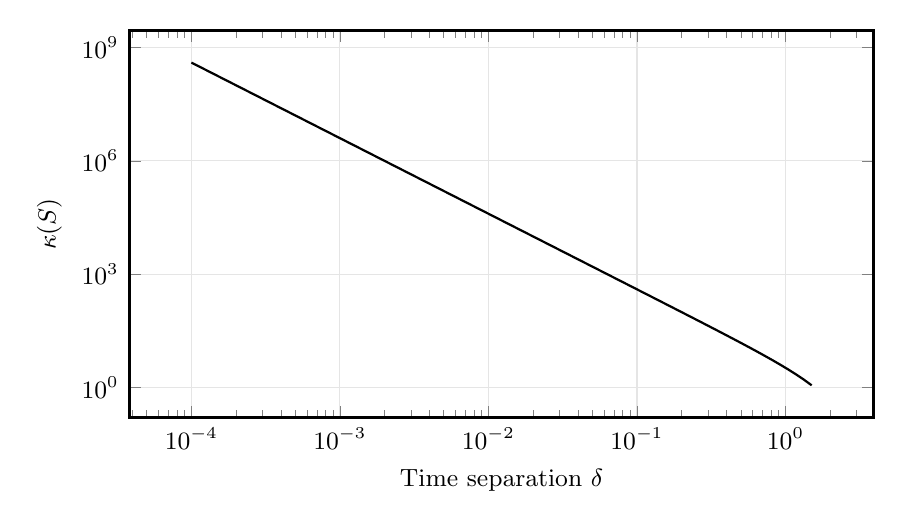
\begin{tikzpicture}
\begin{loglogaxis}[xlabel={Time separation $\delta$},ylabel={$\kappa(S)$},domain=.0001:1.5,samples=100]
\addplot[thick] coordinates {
(0.0001,399999992.549)
(0.000112771963145,314526836.796)
(0.000127175156715,247317829.051)
(0.000143417920861,194470237.038)
(0.000161735204856,152915272.036)
(0.000182391965613,120239892.569)
(0.00020568700024,94546683.0652)
(0.000231957268104,74343673.5191)
(0.000261582764898,58457701.1541)
(0.000294992019224,45966289.7958)
(0.0003326682912,36144079.5518)
(0.000375156562747,28420707.4504)
(0.000423071420677,22347688.0524)
(0.000477105946602,17572369.0568)
(0.000538041742264,13817454.0738)
(0.00060676023529,10864900.229)
(0.000684255428919,8543256.66031)
(0.000771648280117,6717708.62916)
(0.000870202914061,5282249.00565)
(0.000981344909531,4153522.55819)
(0.0011066819197,3265985.65703)
(0.00124802692662,2568100.21722)
(0.00140742446572,2019340.96427)
(0.00158718019977,1587842.18177)
(0.00178989426993,1248547.31197)
(0.00201849890642,981753.955032)
(0.00227630084283,771969.777121)
(0.00256702914754,607012.891396)
(0.00289488916418,477304.471981)
(0.00326462334132,375312.524189)
(0.00368157983129,295114.511917)
(0.00415178985049,232053.44375)
(0.00468205492005,182467.447712)
(0.00528004524886,143477.13127)
(0.00595441068207,112818.378847)
(0.00671490581988,88710.8776541)
(0.00757253111641,69754.7373073)
(0.00853969199973,54849.200065)
(0.00963037831462,43128.7212964)
(0.0108603666837,33912.7084594)
(0.0122474487139,26666.0000025)
(0.0138116883498,20967.7892483)
(0.0155757120956,16487.1887121)
(0.017565036304,12964.0159074)
(0.0198084362671,10193.684897)
(0.0223383624467,8015.32626074)
(0.0251914098656,6302.44562316)
(0.0284088474493,4955.57829434)
(0.0320372149754,3896.5134881)
(0.0361289962647,3063.75272622)
(0.0407433783522,2408.93870396)
(0.0459471076193,1894.04724597)
(0.0518154552706,1489.17929327)
(0.0584333061211,1170.82470479)
(0.0658963864432,920.497054973)
(0.0743126486335,723.660151654)
(0.083803832729,568.883938868)
(0.0945072273591,447.180768745)
(0.106577655607,351.483500814)
(0.120189714501,276.235122597)
(0.135540300541,217.066061324)
(0.152851457773,170.540448681)
(0.172373589626,133.956604532)
(0.194389080965,105.190153968)
(0.219216382743,82.5706677056)
(0.247214618355,64.7846625051)
(0.2787887783,50.799328978)
(0.314395578316,39.8025577664)
(0.354550065708,31.1557815029)
(0.39983306943,24.3568941634)
(0.450899601699,19.0110946138)
(0.508488332648,14.8079613196)
(0.57343227509,11.503427045)
(0.646670833925,8.90560695755)
(0.729263394503,6.8636573911)
(0.822404646478,5.25901864591)
(0.927441864828,3.99853388113)
(1.04589439799,3.00904552047)
(1.17947564504,2.23315715814)
(1.33011783973,1.62591806203)
(1.5,1.15224369639)
};
\end{loglogaxis}
\end{tikzpicture}
\end{center}
\textit{Derived curve for the exact two-state example. Large condition number reflects coordinates, not an inherent singularity of the physical Hamiltonian.}

\section{Canonical orthogonalisation, step by step}
First Hermitian-symmetrise estimated matrices when necessary:
\begin{equation}
\widehat H\leftarrow(\widehat H+\widehat H^\dagger)/2,\qquad
\widehat S\leftarrow(\widehat S+\widehat S^\dagger)/2.
\end{equation}
Diagonalise $\widehat S=V\Lambda V^\dagger$. Choose a cutoff and retain positive eigenvalues satisfying $\lambda_j>\tau_S\lambda_{\max}$. Let
\begin{equation}
W=V_{\rm keep}\Lambda_{\rm keep}^{-1/2}.
\end{equation}
Then $W^\dagger\widehat S W=I$. Solve the ordinary Hermitian problem
\begin{equation}
(W^\dagger\widehat H W)y=Ey,\qquad c=Wy.
\end{equation}
Do not explicitly invert $S$. Do not divide by negative or tiny estimated Gram eigenvalues. Record the retained rank, cutoff, discarded spectrum, and how the result changes across a reasonable cutoff range.

The cutoff trades variance against subspace bias. A large cutoff discards noise-sensitive directions but can also remove useful correlation. A tiny cutoff preserves directions but may amplify measurement error. No single threshold is universally optimal, and choosing it to match a known FCI answer leaks benchmark information.

\section{How matrix noise moves an energy}
For a simple exact generalised eigenpair normalised by $c^\dagger Sc=1$, first-order perturbation gives
\begin{equation}\label{eq:perturb}
\delta E\approx c^\dagger(\delta H-E\delta S)c.
\end{equation}
When $S$ is ill-conditioned, a normalised physical vector may require large Euclidean coordinate norm $\norm c$. This is the mechanism by which small entrywise errors can produce large energy errors.

A $\pm1$ measurement with expectation $\mu$ has empirical-mean variance $(1-\mu^2)/N\le1/N$. This is an \emph{entry-estimation} statement, not a complete eigenvalue error bar. Matrix correlations, conditioning, truncation, and any mitigation must be propagated through the full solve.

Noisy matrices can violate $\widehat S\succeq0$ and can yield apparent energies below the exact target ground energy. Such an estimate is not a variationally valid physical state energy merely because a generalised eigensolver returned it. The laboratory explicitly demonstrates this possibility using binomial measurement noise, not an invented hardware noise model.

\section{Practical diagnostics}
Track Hermiticity defects, Gram eigenvalues, effective rank, the normalisation $c^\dagger Sc$, and the projected residual. In simulation, additionally form the physical vector and its true target energy and full residual. Repeat the complete noisy reconstruction across independent trials.

A single smooth energy curve is not enough. An unstable result can look accurate at one cutoff by chance; a stable result can stagnate because the retained subspace lacks the ground state. Distinguish numerical stability from physical expressiveness.

\checkpoint{At $\delta=0.02$, why can two noiseless states still recover $E_0=-1$ while finite-shot reconstruction performs badly? What happens if thresholding keeps only one Gram mode?}

\chapter{Sample-based Krylov diagonalisation: a different final space}\label{ch:skqd}
\src{The sampled-space idea is established SKQD literature \cite{yu}, related to quantum-selected CI \cite{kanno} and sample-based quantum diagonalisation \cite{robledo}. [M], Section 3.4 applies it with a compact driver and connected expansion. Derivations and counterexamples here are added teaching material.}

\section{Two spaces, two roles}
Prepare several states
\begin{equation}
\ket{\psi_k}=\e^{-\I\Hd t_k}\ket r
=\sum_b\alpha_{kb}\ket b.
\end{equation}
A computational-basis measurement returns $b$ with probability $p_k(b)=\abs{\alpha_{kb}}^2$. Pool the observed labels, deduplicate them, apply the declared selection rules, and obtain a set $\Dset$.

The coherent space and sampled space are
\begin{align}
\mathcal V_Q&=\operatorname{span}\{\ket{\psi_0},\ldots,\ket{\psi_{K-1}}\},\\
\mathcal V_D&=\operatorname{span}\{\ket b:b\in\Dset\}.
\end{align}
They are not generally equal. The first is spanned by at most $K$ coherent states. The second has dimension $D=\abs\Dset$, which may exceed $K$ considerably.

\begin{idea}[What is kept and what is discarded]
SKQD keeps \emph{which configurations were observed}, possibly using counts to choose them. It does not infer the original quantum amplitudes or their phases. The final coefficients are obtained by diagonalising the known target Hamiltonian, not by taking square roots of the observed frequencies.
\end{idea}

\section{Why the overlap becomes the identity}
Let $B_\Dset=[\ket{b_1}\ \cdots\ \ket{b_D}]$. Because the selected bitstrings are distinct,
\begin{equation}
B_\Dset^\dagger B_\Dset=I_D.
\end{equation}
The energy minimisation is therefore
\begin{equation}\label{eq:skqdRitz}
\boxed{\HD c=Ec,\qquad\HD=B_\Dset^\dagger\Ht B_\Dset.}
\end{equation}
Counts do not appear in the overlap matrix. A state observed 200 times and one observed twice each contribute one basis vector if both are retained. Duplicate labels are not additional directions.

The overlap condition number is exactly one, but the \emph{eigenvalue problem} has not become insensitive to everything. Small target spectral gaps can make eigenvectors sensitive; missing configurations cause subspace bias; huge $D$ causes classical cost. $\kappa(S)=1$ eliminates one specific coordinate-conditioning problem.

\section{A subtle example: why these are not the same subspace}
Let $H=X$ and start from its \emph{excited} eigenstate $\ket+$. Real-time evolution only changes a global phase. A conventional single-reference QKS span remains $\operatorname{span}\{\ket+\}$ and returns $+1$.

However, measuring $\ket+$ in the computational basis can reveal both $\ket0$ and $\ket1$. Diagonalising $X$ in their two-dimensional span gives $-1$ and the ground state $\ket-$. SKQD can therefore succeed in this example even though the coherent reference has zero ground-state overlap.

This does not invalidate overlap assumptions in general SKQD convergence results: those assumptions are \emph{sufficient conditions for guaranteed discovery}, not necessary conditions for every individual instance. Nor does it invalidate the polynomial-Krylov obstruction: sampling changed the final subspace.

\section{When can the sampled space contain the coherent space?}
If $\Dset$ contains \emph{every} nonzero computational-basis component of every $\ket{\psi_k}$, then every $\ket{\psi_k}$ lies in $\mathcal V_D$, and thus $\mathcal V_Q\subseteq\mathcal V_D$. With exact projections, $E_D\le E_Q$ follows from the variational principle.

Finite samples usually do not establish complete support. Many amplitudes may be extremely small, so the set of all nonzero components can be exponentially large. Consequently, there is no universal ordering between a practical finite-sample SKQD result and a practical coherent-QKS result.

\section{Constructing a Pauli-space block without the full matrix}
For each Pauli string, define bit masks $x_\ell$ for its $X/Y$ positions and $z_\ell$ for its $Y/Z$ positions. Let $n_Y(P_\ell)$ be its number of $Y$ factors. Then
\begin{equation}\label{eq:pauliaction}
P_\ell\ket b=\I^{n_Y(P_\ell)}(-1)^{\operatorname{popcount}(b\mathbin{\&}z_\ell)}\ket{b\oplus x_\ell}.
\end{equation}
The target label is obtained by XOR; the sign and complex phase are computed explicitly. Use a hash map from selected labels to row indices. For every selected column $b$ and every term, add the contribution only when $b\oplus x_\ell$ is also selected.

This takes $O(LD)$ label lookups for $L$ terms, apart from bit-operation costs, instead of constructing all $2^n$ columns. Dense storage of the final block still costs $O(D^2)$; sparse assembly or matrix-free multiplication is preferable when appropriate. In an untapered determinant basis, Slater--Condon connectivity offers an alternative implementation.

\textbf{Phase check.} $Y\ket0=\I\ket1$ and $Y\ket1=-\I\ket0$. Dropping the factor $\I^{n_Y}$ can silently change the Hamiltonian, even though the observed bit flips look correct. The laboratory tests both real and complex Pauli terms against dense Kronecker products.

\section{The variational guarantee that survives noisy sampling}
For any selected set in the \emph{correct target space}, an exact Hermitian block gives $E_D\ge E_0$. This remains true even if the labels were discovered through a noisy quantum distribution or a classical random procedure. Noise changes the selected subspace, not the algebraic variational principle.

If $\Dset_1\subseteq\Dset_2$ and all other choices remain fixed, $E(\Dset_2)\le E(\Dset_1)$. Thus adding valid low-probability or noise-discovered configurations cannot worsen the exact Ritz energy. Filtering can increase the energy by reducing the space. It may still help memory, reproducibility, or target-sector purity, but it is not automatically an energy improvement.

The qualification ``correct target space'' is essential. A computational bitstring is always a valid qubit basis state, but may belong to the wrong electron-number sector. A lower energy in the wrong sector is not the desired chemistry solution.

\section{A clean support-to-energy bound}
Suppose $\ket g$ is a normalised target ground state and $P_D=B_DB_D^\dagger$. Define captured ground-state weight
\begin{equation}
\alpha=\bra gP_D\ket g>0.
\end{equation}
The normalised projection $\ket q=P_D\ket g/\sqrt\alpha$ lies in the selected space and satisfies $\abs{\braket gq}^2=\alpha$. Let $W=E_{\max}-E_0$ be the target spectral width. Expanding $q$ in energy eigenstates gives
\begin{equation}\label{eq:captured}
\boxed{0\le E_D-E_0\le\bra qH\ket q-E_0\le W(1-\alpha).}
\end{equation}
This is an elementary conditional bound: it tells us why capturing important ground-state support is sufficient. It does \emph{not} tell us that the sampling driver discovers that support, nor does a finite observed histogram directly provide $\alpha$.

For any normalised trial vector of energy $E$ and a nondegenerate ground state with gap $\Delta>0$,
\begin{equation}
1-\abs{\braket g\psi}^2\le\frac{E-E_0}{\Delta}.
\end{equation}
Near a small gap, accurate energy can coexist with modest wavefunction fidelity. In a degenerate ground space, replace overlap with projection onto that whole space.

\checkpoint{Why can noisy SKQD sampling remain variational while noisy QKS matrix reconstruction can return an energy below $E_0$? State all representation and sector assumptions needed.}

\chapter{Sampling theory: what finite shots can and cannot discover}\label{ch:sampling}
\src{Probability calculations and resource objectives are derived here. General SKQD convergence under sparsity, overlap, and spectral assumptions is discussed in Yu et al. \cite{yu}; that theorem must not be automatically applied to an arbitrary pruned driver.}

\section{One configuration, one distribution}
For a configuration with probability $p$, $N$ independent shots give a binomial count $C$. The probability of observing it at least once is
\begin{equation}
\Pr(C\ge1)=1-(1-p)^N.
\end{equation}
To make the probability of missing it at most $\delta$, choose
\begin{equation}
N\ge\frac{\log\delta}{\log(1-p)}\simeq\frac{\log(1/\delta)}p\quad(p\ll1).
\end{equation}
The scale $1/N$ is therefore a heuristic detectability scale, not a sharp cutoff.

For $p=0.001$ and $N=1024$,
\begin{equation}
\Pr(C\ge1)=0.6410285,\qquad\Pr(C\ge2)=0.2730738.
\end{equation}
A configuration at $0.1\%$ probability is not reliably discovered by one 1024-shot circuit, and requiring two counts makes retention substantially less likely. At $p=10^{-6}$, about $3.0\times10^6$ independent shots give a $95\%$ chance of seeing \emph{one specified configuration once}; finding many configurations or requiring repeated observations costs more.

\begin{center}
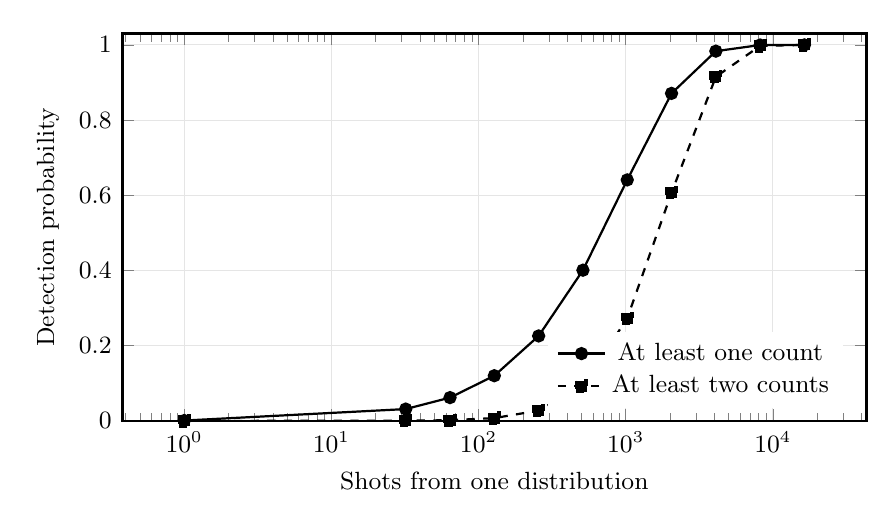
\begin{tikzpicture}
\begin{semilogxaxis}[xlabel={Shots from one distribution},ylabel={Detection probability},ymin=0,ymax=1.03,legend pos=south east]
\addplot[thick,mark=*] coordinates {(1,0.001) (32,0.0315089242405) (64,0.0620250361742) (128,0.120202967236) (256,0.225957181139) (512,0.40085771457) (1024,0.64102852181) (2048,0.871139477846) (4096,0.98339496583) (8192,0.99972427284) (16384,0.999999923975)};
\addlegendentry{At least one count}
\addplot[thick,dashed,mark=square*] coordinates {(1,8.67361737988e-19) (32,0.000486187079007) (64,0.00193454800113) (128,0.00747622029516) (256,0.0276038661963) (512,0.0937897965125) (1024,0.273073773396) (2048,0.606968957956) (4096,0.915312663569) (8192,0.997463254929) (16384,0.999998677126)};
\addlegendentry{At least two counts}
\end{semilogxaxis}
\end{tikzpicture}
\end{center}
\textit{Binomial calculation for $p=0.001$; plotted coordinates are rounded. Exact values are in the laboratory CSV.}

\section{Several times and nonuniform shot allocation}
For independent circuit executions with probabilities $p_k(b)$ at time $t_k$ and shot counts $N_k$,
\begin{equation}\label{eq:miss}
\Pr(b\text{ never observed})=\prod_{k=0}^{K-1}(1-p_k(b))^{N_k}
\le\exp\left[-\sum_kN_kp_k(b)\right].
\end{equation}
Multiple times help when their distributions expose different configurations. They can also be redundant. Increasing the number of times at fixed total shots is not guaranteed to help, because it reduces sampling at every individual time.

If $L_*$ important labels each satisfy $\sum_kN_kp_k(b)\ge\log(L_*/\delta)$, a union bound gives probability at least $1-\delta$ that all are observed. This condition refers to the \emph{actual sampled distributions}, not to the exact ground-state probabilities.

\section{Why high ground-state weight does not ensure high sampling probability}
The sampling amplitude is
\begin{equation}
\alpha_{kb}=\bra b\e^{-\I\Hd t_k}\ket r.
\end{equation}
The ground-state coefficient is $\braket b g$ for the target $\Ht$. These quantities can be very different, especially when $\Hd\ne\Ht$. A determinant important in the ground state may be nearly absent at all chosen times; a frequent sampled determinant may matter little to the target energy.

At short time,
\begin{equation}
\bra b\e^{-\I\Hd t}\ket r=-\I t(\Hd)_{br}+O(t^2)\qquad(b\ne r),
\end{equation}
for a coordinate reference. Directly coupled states initially appear with probability $t^2\abs{(\Hd)_{br}}^2$. An indirectly connected state may first appear at a higher power of $t$ and thus be much harder to sample. Interference can suppress it again at particular later times.

\section{Sparsity is basis-dependent}
A state is useful for sample-based methods when most relevant weight is concentrated on a manageable number of basis configurations. This is not the same as saying the Hamiltonian is sparse. A sparse matrix can have a dense ground eigenvector.

Changing orbitals or the qubit basis can alter how concentrated the ground state is. It also changes the driver, matrix elements, state preparation, and sometimes tapering symmetries. A claim about sparsity must specify the representation and the retained-weight tolerance, not merely the number of qubits.

The SKQD literature provides conditional convergence results rather than a generic polynomial-time solution to arbitrary molecular ground-state problems \cite{yu}. Their assumptions include favourable reference overlap, suitable spectral scales, and sufficient concentration and accessibility of important configurations. Ankush's compact driving approximation adds a separate empirical question: does that cheaper generator preserve useful discovery probabilities?

\section{Statistical filtering is a selection rule, not a noise detector}
A rare valid excitation and a rare noise-generated label can have identical observed counts. Conversely, a systematic error can produce a frequent wrong label. Frequency alone does not identify the physical origin of an event.

For a per-circuit threshold $C\ge q$,
\begin{equation}
\Pr(\text{retained})=1-\sum_{c=0}^{q-1}\binom Nc p^c(1-p)^{N-c}.
\end{equation}
A maximum-over-times rule uses the probability that at least one circuit passes its threshold. When shot counts differ, define the count and frequency conditions \emph{jointly for each circuit}; do not combine the highest count from one circuit with the highest frequency from a different one unless that is deliberately the policy.

In [M], $N=1024$, $N_{\min}=2$, and $\nu_{\min}=0.001$. Since $\lceil1024\times0.001\rceil=2$, the two tier-1 inequalities impose the same integer threshold for equal shots. They are not two statistically independent checks.

\section{How to estimate uncertainty honestly}
The final energy is a nonlinear, often discontinuous function of counts because labels enter or leave the selected set. Repeated experiments or independent multinomial resampling in simulation are more informative than an error bar on one mean count.

A bootstrap of observed counts cannot discover configurations missing from every original sample. It estimates variation conditional on the observed support and may underestimate unseen-support uncertainty. Track discovery saturation, independent held-out batches, subspace size, threshold sensitivity, and energy/residual changes. An energy plateau alone is not a proof that no important configuration remains undiscovered.

\checkpoint{Derive Eq.~\eqref{eq:miss}. Why is substituting the exact ground-state probability into that equation unjustified for an arbitrary compact driver?}

\chapter{Ankush's four reductions, reconstructed carefully}\label{ch:reductions}
\src{This chapter follows [M], Sections 3.1--3.5, in their original order. Each reported step is separated from its mathematical conditions and implementation questions.}

\section{First distinguish the Hamiltonians}
The full molecular model, its active-space model, its exactly tapered representation, its pruned approximation, and its compact driver are not one interchangeable object. A precise chain is
\begin{equation}
H_{\rm molecule}\longrightarrow H_{\rm active}
\xrightarrow{\text{sector isometry }V_s}\Ht=V_s^\dagger H_{\rm active}V_s
\longrightarrow H_{\rm pruned}\longrightarrow\Hd.
\end{equation}
The first arrow can introduce model error. The isometric sector reduction is exact for that sector. The last two arrows are approximations used for circuit design. The final selected-space projection should use $\Ht$, not the pruned Hamiltonian, and should include all target constant-energy offsets.

\begin{sourcebox}
{[M]}, Eqs. (30)--(34), uses a compact $H_{\rm drive}$ for time evolution and a ``full untruncated'' $H_{\rm full}$ for classical matrix construction. In these notes, that latter operator is denoted $\Ht$ to emphasise that it must be expressed in the same active-space/tapered representation as the sampled basis.
\end{sourcebox}

\section{Reduction 1: exact $Z_2$ symmetry tapering}
A Pauli symmetry $\tau$ satisfies $\tau^2=I$ and commutes with every Hamiltonian term. Its eigenvalues are $\pm1$. Selecting a known joint symmetry sector can remove qubits used only to encode these fixed eigenvalues.

Write a Pauli string, up to phase, as a binary vector $(x\mid z)\in\mathbb F_2^{2n}$. Two such strings commute exactly when
\begin{equation}
x\cdot z'+z\cdot x'=0\pmod2.
\end{equation}
Assemble one row per Hamiltonian Pauli term into $G$. With $\Omega=\begin{psmallmatrix}0&I\\I&0\end{psmallmatrix}$, the commuting-Pauli condition is
\begin{equation}
G\Omega v_\tau^T=0\pmod2.
\end{equation}
The nullspace gives candidates. One must then choose an \emph{independent mutually commuting} set of sector generators. Nullspace vectors need not all commute with one another, and arbitrary candidates cannot all be fixed simultaneously. General tapering theory is established prior work \cite{bravyi}.

A Clifford change of basis maps suitable generators to single-qubit Pauli operators. The manuscript writes factors $(\tau_i+X_{q_i})/\sqrt2$. Such a factor is unitary when $\tau_i$ and $X_{q_i}$ anticommute; the full construction also requires compatible generator and pivot choices. Those conditions are necessary, not optional details.

If $U$ maps the selected symmetries to pivot-$X$ operators and $\ket{s_X}$ is the fixed joint eigenstate on the removed qubits, define the embedding
\begin{equation}\label{eq:isometry}
V_s\ket b=U^\dagger(\ket{s_X}\otimes\ket b),\qquad V_s^\dagger V_s=I.
\end{equation}
Then $\Ht=V_s^\dagger H_{\rm active}V_s$ is the reduced target. This formula makes both spectral preservation and basis interpretation explicit.

\subsection{A complete two-qubit tapering example}
Consider
\begin{equation}
H=gX_0X_1+h(Z_0+Z_1)+JZ_0Z_1.
\end{equation}
It commutes with $Z_0Z_1$. In the even-parity sector, choose $V\ket0=\ket{00}$ and $V\ket1=\ket{11}$. Direct substitution yields
\begin{equation}
V^\dagger HV=gX+2hZ+JI.
\end{equation}
The two even-sector energies are $J\pm\sqrt{g^2+4h^2}$. The odd sector is a different problem. Replacing the sector sign incorrectly can produce a perfectly accurate answer for the wrong sector.

\subsection{After tapering, bitstrings need not be determinants}
Before Jordan--Wigner tapering, occupation labels and determinant labels coincide. After a general Clifford transformation, $V_s\ket b$ can be a superposition of determinants. [M] explicitly states this on page 7, although later passages use the word ``determinants'' for reduced basis states.

For example, the $+1$ sector of $X_0X_1$ can use $(\ket{00}+\ket{11})/\sqrt2$ and $(\ket{01}+\ket{10})/\sqrt2$ as orthonormal embedded basis states. Neither is a single occupation determinant. Nevertheless,
\begin{equation}
\braket{V_sb_i}{V_sb_j}=\delta_{ij},
\end{equation}
so $S=I$ remains correct in the reduced basis.

Do not count electrons by the Hamming weight of an arbitrary tapered bitstring. Transform the particle-number operator as $N_s=V_s^\dagger\hat N V_s$, or use an explicitly validated encoding map. Fixed parity does not generally fix exact particle number.

\begin{sourcebox}
{[M]}, Section 3.2, reports four removed qubits for water/methane and five for several other examples. It also states that sectors are scanned against an exact active-space benchmark. That is the reported validation procedure; it is not a scalable, benchmark-free method of selecting an unknown physical ground sector.
\end{sourcebox}

\section{Reduction 2: Epstein--Nesbet-inspired term pruning}
The manuscript separates the tapered Pauli Hamiltonian into all-$I/Z$ diagonal terms and off-diagonal terms containing $X/Y$. It preserves the diagonal part and estimates importance of off-diagonal terms using a second-order energetic score, with reported pruning threshold $\eta_{\rm prune}=10^{-7}$ Ha \cite{kumar}.

For a reference coordinate state with diagonal energy $\epsilon_r=H_{rr}$ and a candidate $b$ with diagonal energy $\epsilon_b=H_{bb}$, ordinary second-order perturbation theory suggests
\begin{equation}\label{eq:EN}
\Delta E^{(2)}=\sum_{b\ne r}\frac{|H_{br}|^2}{\epsilon_r-\epsilon_b}.
\end{equation}
When $\epsilon_b>\epsilon_r$, each contribution is negative. A magnitude score is $|H_{br}|^2/|\epsilon_b-\epsilon_r|$. For one isolated Pauli coupling, its numerator reduces to the coefficient squared times the relevant unit-modulus phase.

\begin{caution}[What this score is not]
It is not an exact contribution of each Pauli term to the correlated ground energy. Several terms may connect the same pair of configurations, and their amplitudes add \emph{before} squaring. Higher-order paths matter, and small denominators invalidate a simple weak-coupling interpretation. A per-term cutoff alone does not prove a bound on the total omitted correlation.
\end{caution}

Indeed,
\begin{equation}
\left|\sum_{\ell:\,r\to b}h_\ell\omega_\ell(r)\right|^2
\ne\sum_{\ell:\,r\to b}|h_\ell|^2
\end{equation}
in general. Two large contributions can cancel. Individual Pauli pruning can also break exact particle-number conservation even if the original grouped fermionic excitation conserves it. For example $X_0X_1+Y_0Y_1$ conserves the total occupation of two modes; $X_0X_1$ alone does not.

Keeping the full diagonal target avoids one obvious source of energy-model drift. But the bound $|\delta E|\le\sum_{\ell\in\mathrm{removed}}|h_\ell|$ is a conservative operator-norm estimate, not a statement that all diagonal errors must add constructively. Removing an identity term from the \emph{driver} only changes a global phase; removing it from the \emph{reported target energy} shifts every answer.

\section{Reduction 3: compact driver and ancilla-free sampling}
\begin{sourcebox}
{[M]}, Section 3.4.3, ranks terms by $|c_j|$ and writes
\[
\Hd=H_{\rm diag}+\sum_{j=1}^{L_{\rm drive}}c_jP_j,
\quad t_k\in\{0,0.15,0.30,0.45,0.60,0.75\}.
\]
The prose suggests 10--30 drive terms, while Table 3 gives 80 for nitrogen and 50 for methane. Thus 10--30 is not a universal setting. The time-unit convention and exact selected terms are needed for replication.
\end{sourcebox}
The driver is a \emph{proposal mechanism for useful support}. Accuracy of its time-evolved state relative to full-target evolution is not the final objective. Conversely, a driver can have small-looking coefficients yet completely disconnect an important configuration component. In that case additional shots cannot reveal the disconnected states.

The reference must also be transformed consistently. A Hartree--Fock occupation bitstring before tapering need not remain a simple bitstring after the Clifford map. One must provide the reduced reference preparation, not assume it is unchanged.

\subsection{Connected expansion}
The manuscript's Eq. (33) uses one graph neighbourhood of the retained core:
\begin{equation}\label{eq:expand}
\Dset_{\rm active}=\Dset_{\rm core}\cup
\{b:\exists a\in\Dset_{\rm core},\ |(\Ht)_{ab}|\ge\epsilon_{\rm expand}\}.
\end{equation}
This is a classical operation. Its output depends on the threshold, symmetry restrictions, whether one or several shells are taken, whether new states are filtered again, and any dimension cap. The numerical expansion threshold is not specified in the uploaded manuscript.

The correct final projection is $\HD=B_D^\dagger\Ht B_D$. All target couplings \emph{between included basis vectors} are restored. Couplings to excluded vectors are not incorporated by ordinary subspace diagonalisation.

\begin{caution}[Restored terms are not restored missing states]
{[M]} says omitted correlation is fully recovered through connected expansion and full-Hamiltonian projection. The precise mathematical statement is narrower: full target matrix elements are restored \emph{within the selected space}. Missing important configurations can still produce error. Chapter~\ref{ch:lab} gives an explicit counterexample with a nonzero external residual.
\end{caution}

\section{Reduction 4: the two-tier filter}
The reported statistical rule retains labels whose maximum count and frequency pass $N_{\min}=2$ and $\nu_{\min}=0.1\%$ (typical settings). The energetic rule then uses
\begin{equation}\label{eq:energyfilter}
I_b=\frac{|\bra{\Phi_0}\Ht\ket b|^2}
{|\bra{\Phi_0}\Ht\ket{\Phi_0}-\bra b\Ht\ket b|}
\end{equation}
with a reported threshold of $10^{-6}$ Ha. In [M] this is coupled to the Hartree--Fock reference rather than to the final correlated Ritz vector.

A replication must specify how it treats the reference itself, zero/small denominators, states with zero direct reference coupling, and transformed references that are not coordinate states. In the teaching code, the reference is explicitly protected; that is a stated safety policy, not an undocumented reconstruction of Ankush's code.

\textbf{Why a zero score need not mean noise.} In the chain of Eq.~\eqref{eq:chain}, configuration 2 has $H_{02}=0$, so the reference-coupling score is zero. But $H_{12}\ne0$, and the ground state has nonzero weight on configuration 2. A correlated path can be important even when a single-reference energetic filter rejects it. Connected expansion may reintroduce it if its parent survives, but this is not a universal guarantee.

The paper's claim that filtering removes noise without discarding physical multireference configurations requires evidence beyond the filtering formulas themselves. A useful validation would report which known valid configurations are falsely rejected, how much ground-state weight is lost, and the resulting accuracy--dimension tradeoff.

\checkpoint{Draw two arrows: $H_{\rm drive}\to$ sampling and $H_{\rm tar}\to$ classical projection. Explain what is exact in tapering, what is approximate in pruning, and what remains unknown after support selection.}

\chapter{Molecular results: what Ankush reports}\label{ch:results}
\src{All molecular energies, gate counts, and execution labels in this chapter are transcribed from [M], Sections 4--5 and Tables 1--3. None is an independently reproduced result. Ratios and dimension checks are explicitly derived here.}

\section{The water workflow, step by step}
The reported water geometry is $R=1.0$ \AA\ and bond angle $104.5^\circ$, using STO-3G. Table 3 identifies CAS$(8e,6o)$. The active representation starts with 12 spin orbitals, and the reported symmetry reduction leaves 8 qubits.

The quantum stage uses six time points and 1024 shots at each, for 6144 executions. Section 4.1 identifies physical Quantinuum H2-1 execution and provides the job identifier
\begin{center}\small\ttfamily 3c925cba-e92a-4124-84dc-cd1c64fdf5c4\end{center}
A job identifier documents the claim's intended provenance, but without an accessible export it does not independently verify the job content.

\begin{center}
\begin{tabularx}{\linewidth}{@{}p{44mm}Y@{}}
\toprule Stage & Reported water setting or output\\\midrule
Molecular model & STO-3G, $R=1.0$ \AA, $104.5^\circ$; CAS$(8e,6o)$ in Table 3.\\
Register & 12 spin orbitals $\to$ 8 tapered qubits.\\
Sampling & 6 circuits $\times$ 1024 shots $=6144$.\\
Native resources & 150 ZZPhase, 356 $R_z$, 318 PhasedX; stated total 833 gates; depth 428.\\
Raw support & 101 unique bitstrings.\\
Filtered core & 53 retained after two-tier filtering.\\
Expanded filtered space & 249 objects called ``determinants'' by [M].\\
Raw final energy & $-75.019670$ Ha; reported error $0.1113$ mHa.\\
Filtered final energy & $-75.019473$ Ha; reported error $0.3095$ mHa.\\\bottomrule
\end{tabularx}
\end{center}

The raw and filtered branches are different post-processing routes. The source gives 249 as the \emph{filtered expanded} dimension; it does not give the corresponding raw expanded dimension. Do not assume both final spaces have equal size.

The raw branch has the lower reported error. That is compatible with variational support selection: additional valid configurations can improve the Ritz energy. It does not demonstrate that hardware noise intrinsically improves chemistry. Random discovery, different final subspaces, and filtering choices must be separated.

\section{What the conventional-QKS comparison does and does not show}
\begin{center}
\small
\begin{tabularx}{\linewidth}{@{}Yrrrr@{}}
\toprule Reported method & Qubits & ZZPhase & Depth & Error (mHa)\\\midrule
Unpruned standard QKS &12&5436&18572&$>50$\\
Statevector SKQD &8&150&428&0.1836\\
1024-shot H2-1E &8&150&428&0.1836\\
Physical H2-1, raw &8&150&428&0.1113\\
Physical H2-1, filtered &8&150&428&0.3095\\\bottomrule
\end{tabularx}
\end{center}
\textit{Transcribed from [M], Table 1. Its unpruned baseline is labelled as decohering. These are not new measurements or an independently verified paired experiment.}

This is evidence for the manuscript's \emph{combined pipeline comparison as reported}. It is not a clean isolation of the sampled-versus-coherent diagonalisation choice: tapering, drive truncation, circuit structure, measurement protocol, and classical expansion all change. A fair algorithmic ablation should give competing methods the same exact reductions where applicable and disclose different output tasks and classical workloads.

The table also leaves implementation questions: does the standard-QKS qubit count include an ancilla; what time/step determines the quoted depth; were gates averaged across times; and how was the $>50$ mHa baseline obtained? Those details cannot be recovered from the table alone.

\section{The most revealing dimension check}
An 8-qubit register has dimension $2^8=256$. Thus the reported 249-state filtered expansion is
\begin{equation}
\frac{249}{256}=0.97265625\simeq97.3\%
\end{equation}
of the \emph{entire tapered computational-basis dimension}.

\begin{idea}[Why this observation matters]
If those 249 labels are reduced computational-basis states, the final classical diagonalisation is nearly full-space diagonalisation of an 8-qubit target. Very high accuracy is then unsurprising. This does not negate the hardware demonstration, but it makes the quantum contribution to \emph{basis discovery} a question to test, not a conclusion to assume.
\end{idea}

There is a second check. Under the usual balanced-spin CAS$(8e,6o)$ sector, there are only 225 distinct occupation determinants. Therefore 249 cannot denote 249 distinct orthonormal occupation determinants all inside that fixed $(N_\alpha,N_\beta)=(4,4)$ sector. Plausible interpretations include a larger parity-sector coordinate basis or a different counting convention. The manuscript's page-7 warning about symmetry-adapted combinations is relevant, but does not by itself specify the implemented sector restriction.

Ask for the reduced basis map, the transformed number/spin operators, the actual selected labels, and the precise space over which the reference eigenvalue was computed. Do not resolve this ambiguity by silently treating tapered Hamming weight as electron number.

\section{Fluorine and the wider suite}
For F$_2$ at $R=1.41$ \AA, Section 4.3 reports CAS$(10e,6o)$, 12 to 7 qubits, 220 pruned Pauli terms, an average of 153.3 ZZPhase gates, depth 505, and physical H2-2 execution. The reported energy is $-196.041436$ Ha with $0.0000$ mHa error relative to CASCI.

A displayed zero means agreement at the reported precision, not an exact symbolic equality. Request unrounded energies, final space dimensions, solver tolerances, and independent repetitions. The balanced-spin CAS target contains 36 determinants before additional symmetry restrictions; this is not a classically intractable eigenproblem.

\begin{center}
\small
\begin{tabularx}{\linewidth}{@{}lYrrr@{}}
\toprule Molecule & Active space & Qubits & Drive terms & Max error (mHa)\\\midrule
H$_2$O & CAS$(8e,6o)$ &8&10--30&0.3095\\
F$_2$ & CAS$(10e,6o)$ &7&30&0.0000\\
N$_2$ & CAS$(6e,6o)$ &7&80&0.2854\\
CH$_4$ & CAS$(6e,6o)$ &8&50&0.0016\\
C$_2$H$_4$ & CAS$(2e,2o)$ &4&10&0.0000\\
C$_6$H$_6$ & CAS$(6e,6o)$ &7--8&20&0.0012\\\bottomrule
\end{tabularx}
\end{center}
\textit{Source: [M], Table 3. The source reports a 100\% pass rate across its benchmark suite. The uploaded file does not provide a per-geometry manifest distinguishing every physical, emulator, and statevector execution.}

The ethylene example uses 11 torsion angles and a very small CAS$(2e,2o)$ model. The benzene example uses 9 geometries in a six-orbital $\pi$ active space. Those are useful controlled targets, but are not the same as solving the full all-electron 72-spin-orbital benzene problem discussed in the manuscript's motivation.

A curve of electronic energies versus a torsion angle is not itself a simulation of nonadiabatic nuclear dynamics. Statements about ``nonadiabatic lag'' require a defined dynamical observable or trajectory; pointwise Born--Oppenheimer ground energies do not establish that property.

\section{An implementation ledger: known, partial, and missing}
\begin{longtable}{@{}p{42mm}p{18mm}p{90mm}@{}}
\toprule Item & Status & What is available or still needed\\\midrule\endhead
Water geometry/basis & Reported & Bond length, angle, and STO-3G appear in Section 4.1.\\
Active spaces & Reported & Table 3 gives CAS labels, but not the full orbital construction.\\
Molecular integrals & Missing & Need one-/two-electron integrals, constant offsets, ordering, and units.\\
Tapering map & Partial & General theory and qubit counts are given; actual generators, Clifford, signs, and reference mapping are absent.\\
Driver & Partial & Ranking rule, broad term counts, and time grid are given; exact coefficients and selected Pauli strings are absent.\\
Product formula & Partial & General formula appears, but exact per-experiment ordering, repetitions, and compilation settings are not supplied.\\
Filters & Partial & Typical count/frequency and energetic thresholds are given; edge cases and operation order are not fully specified.\\
Connected expansion & Partial & Equation (33) gives a rule; numerical threshold, shell count in code, dimension cap, and sector checks are not supplied.\\
Raw measurements & Missing & No complete count file, result metadata, calibration record, or timing export.\\
Benchmarks & Partial & Rounded energies/errors; no full-precision target Hamiltonian/reference manifest.\\
Native resources & Partial & Summary counts/depth; no compiled circuit export or per-time statistics.\\
Classical processing & Missing & No wall time, RAM, eigensolver options, or support-list export for each branch.\\\bottomrule
\end{longtable}

\section{Attribution and the strength of the conclusion}
SKQD itself predates the uploaded October 2026 manuscript: Yu et al.'s preprint appeared in January 2025 \cite{yu}. Quantum Krylov, tapering, and sampled configuration diagonalisation also have established primary literature \cite{stair,bravyi,kanno,robledo}. The manuscript-specific object to evaluate is the \emph{integration, parameter choices, filtering/expansion procedure, compilation, and reported molecular experiments}, not an unsupported claim that all underlying ingredients were first introduced here.

The uploaded source alone does not establish quantum advantage. That requires strong classical baselines for the \emph{same active-space task}, comparable error targets, and full resource accounting. Nor can the general SKQD convergence theorem automatically certify a compact, independently pruned driver.

\checkpoint{Explain why 249/256 is relevant but does not by itself identify the correct electron-number sector. What exact files would resolve the interpretation?}

\chapter{The reproducible laboratory}\label{ch:lab}
\src{All examples in this chapter are independently specified teaching calculations. They do not use Ankush's unavailable molecular integrals, circuits, or hardware samples. Numerical values were checked with the supplied Python program.}

\section{Run the experiments}
From the package directory:
\begin{lstlisting}
python -m pip install numpy scipy matplotlib
python code/krylov_skqd_lab.py --out results --repeats 200
python code/make_figures.py
\end{lstlisting}
The lab fixes random seed 20261008 and writes individual trial data as well as summaries. A different library version can change last-bit results or random-number details; archive the environment when doing research-grade reproduction. The included \texttt{requirements.txt} records the versions used for this package.

The tests check exact QKS energies, conservation of raw real-time energy, variational ordering for nested configuration sets, inaccessible support under a truncated driver, fermionic anticommutation/signs, a known Hubbard-dimer energy, Pauli projection including $Y$ phases, and an exact parity-sector embedding.

\section{Lab A: two-state QKS}
Use $H=Z$ and $\ket r=\ket+$. Sweep the time separation. The function \texttt{qks} constructs $\Phi$, $H_K$, and $S_K$ from exact statevectors, then calls \texttt{canonical\_ritz}. It returns a physical state, retained rank, Gram spectrum, and full residual.

Tasks: verify the $\pm1$ eigenvalues; inspect the growth of $\kappa(S)$; increase the cutoff until a useful direction is removed; and compare the classical coefficient norm with the physical state norm. Remember that a large coordinate vector is not a state-normalisation failure when $c^\dagger Sc=1$.

The separate shot-noise experiment estimates the real and imaginary off-diagonal elements of $S$ and $H_K$ and the two diagonal energy entries using independent $\pm1$ samples. For two states, this accounts for six measurement settings and $6N$ total shots. It is a deliberately transparent synthetic measurement experiment, \emph{not} a Quantinuum error model and not a full compiled resource comparison.

\section{Lab B: restoration is limited by the included space}
Use the target in Eq.~\eqref{eq:chain}, but a driver containing only its diagonal and the $0\leftrightarrow1$ coupling:
\begin{equation}
H_{\rm drive}=\operatorname{diag}(0,0.6,1.0,1.5)
-0.2(\ket0\bra1+\ket1\bra0).
\end{equation}
Starting from $\ket0$, exact driver evolution has zero probability on configurations 2 and 3 at every time. No increase in shots can change that.

Take seed set $\{0,1\}$ and expand under the full target. The verified results are
\begin{center}
\begin{tabular}{@{}rrrrr@{}}
\toprule Shells & $D$ & Ritz energy & Energy error & Full residual\\\midrule
0 &2&$-0.0605551275$&$5.36694\times10^{-3}$&$7.24460\times10^{-2}$\\
1 &3&$-0.0658723616$&$4.97010\times10^{-5}$&$8.78132\times10^{-3}$\\
2 &4&$-0.0659220627$&$<10^{-14}$&$<10^{-14}$\\\bottomrule
\end{tabular}
\end{center}
The eigensolver for each small block is numerically converged. Only the full-space calculation has a vanishing external residual. This is the simplest concrete demonstration of why restoring all \emph{included} matrix elements does not restore every missing correlation path.

\begin{center}
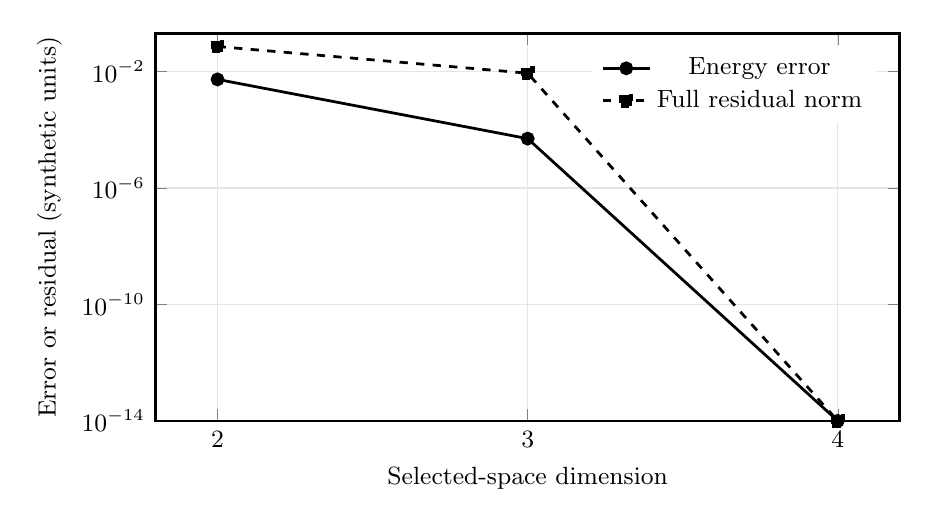
\begin{tikzpicture}
\begin{semilogyaxis}[xlabel={Selected-space dimension},ylabel={Error or residual (synthetic units)},xtick={2,3,4},ymin=1e-14,ymax=.2,legend pos=north east]
\addplot[mark=*] coordinates {(2,.0053669351274)(3,.00004970104254)(4,1e-14)};\addlegendentry{Energy error}
\addplot[dashed,mark=square*] coordinates {(2,.07244603717)(3,.00878131542)(4,1e-14)};\addlegendentry{Full residual norm}
\end{semilogyaxis}
\end{tikzpicture}
\end{center}
\textit{Values below $10^{-14}$ are displayed at $10^{-14}$. The Hamiltonian is synthetic, not molecular water.}

\section{Lab C: finite-shot support discovery and classical controls}
For the same four-state target, now sample exact full-target evolution at times $0,0.4,\ldots,2.0$. Each shot budget has 200 independently drawn replicates. Compare raw support, a count-at-least-two filter, raw support plus one connected shell, and a uniform classical sampling baseline plus the same expansion.

The uniform baseline is intentionally strong in this tiny four-configuration system: it quickly covers the whole space. That is a \emph{feature of the control experiment}, not an embarrassment to hide. It prevents mistaking accurate diagonalisation of a tiny matrix for a quantum sampling advantage.

Read \texttt{sampling\_trials.csv} to see the full outcome distribution, not only its best trial. Increasing a threshold may reduce mean dimension and worsen energy. Adding a shell can dominate the gain from extra shots. Since separate budgets redraw data independently, individual realised curves need not be monotone, although nested exact subspaces obey Eq.~\eqref{eq:nested}.

\section{Lab D: a fermionic example with an analytic answer}
The two-site Hubbard model is a lattice-fermion teaching model, not an ab initio molecule. Use orbitals $(0,1)$ for spin-up on sites $(A,B)$ and $(2,3)$ for spin-down:
\begin{equation}
H=-t(a_0^\dagger a_1+a_1^\dagger a_0+a_2^\dagger a_3+a_3^\dagger a_2)
+U(n_0n_2+n_1n_3).
\end{equation}
In the sector with one up and one down electron, order the basis as
\begin{equation}
\ket{0101},\ \ket{0110},\ \ket{1001},\ \ket{1010}.
\end{equation}
For $t=1$ and $U=4$, the Hamiltonian is
\begin{equation}
H_{\rm sector}=\begin{pmatrix}
4&-1&-1&0\\-1&0&0&-1\\-1&0&0&-1\\0&-1&-1&4
\end{pmatrix}.
\end{equation}
Symmetric combinations of the two doubly occupied and two singly occupied configurations reduce the coupled block to $\begin{psmallmatrix}U&-2t\\-2t&0\end{psmallmatrix}$. Its lower eigenvalue is
\begin{equation}
E_0=\frac{U-\sqrt{U^2+16t^2}}2=2-\sqrt8=-0.828427124746\ldots.
\end{equation}
The remaining symmetry combinations have energies $U$ and 0, so this is the sector ground energy. The code builds the full fermionic operators using parity signs, projects into the four-state sector, and verifies the analytic answer.

\section{Lab E: the functions you can reuse}
\texttt{canonical\_ritz}$(H_K,S,\mathrm{cutoff})$ performs the stable coherent-space solve. \texttt{selected\_ritz}$(H,\mathrm{labels})$ solves an orthonormal coordinate block and returns its full residual for a small dense target. \texttt{projected\_paulis}$(\mathrm{terms},\mathrm{labels})$ builds a selected block without the full Hilbert-space matrix. \texttt{expand}$(H,\mathrm{labels},\mathrm{threshold},\mathrm{shells})$ performs explicitly defined graph expansion. \texttt{sample\_counts} and \texttt{select\_counts} keep sampling and filtering separate.

For large chemistry, replace the dense target used by the teaching helpers with sparse/matrix-free Pauli or determinant connectivity. Do not pass a 50-qubit Hamiltonian to a function that constructs $2^{50}$ amplitudes. The pedagogical dense simulator is a validation tool, not a scalable quantum emulator.

\checkpoint{Modify the chain driver so configuration 2 becomes weakly reachable. Determine how many shots are needed to discover it, and compare that cost with one classical expansion shell.}

\chapter{Reproducing the pipeline without hidden assumptions}\label{ch:repro}
\src{Operational reconstruction based on [M], with explicit added validation steps. Missing source inputs remain marked as missing rather than assigned invented molecule-specific values.}

\section{The experiment contract}
Before coding, write down the target Hamiltonian, sector, energy offset, reference, and desired output. An energy-only estimate, a classical CI coefficient vector, and a quantum circuit preparing the approximate eigenstate are different deliverables.

The minimal reproducible record should contain the molecular geometry in a declared unit, basis and active-orbital specification, integral convention, bit order, mapped/tapered Hamiltonians, symmetry generators and signs, reference map, driving terms, time units and grid, Trotter order/steps, compilation settings, all count files, and classical selection parameters.

A filename such as \texttt{water\_8q.json} is not sufficient provenance. Store an immutable hash of the actual Hamiltonian and circuit input. Include whether constant identity terms were removed only from the driver or also from the energy reference.

\section{A faithful high-level algorithm}
\begin{lstlisting}
INPUT: target Hamiltonian and exact sector map; reference;
       driver; time grid; shot budgets; filter rules;
       connected-expansion policy; numerical tolerances.

1. Validate the active model, sector, bit order, and reference.
2. Compile reference + exp(-i H_drive t_k) for every time.
3. Archive the compiled circuits and resource estimates.
4. Execute the requested shots; archive raw per-time counts.
5. Decode labels in the same representation as H_target.
6. Apply the explicitly specified physical-sector checks.
7. Construct the core using declared count/frequency rules.
8. Apply the declared energetic filter, with edge cases logged.
9. Expand under H_target using the declared threshold/shells.
10. Deduplicate; construct B_D^dagger H_target B_D.
11. Solve the Hermitian eigenproblem and record residuals.
12. Report energy, support sizes, uncertainty, and all costs.

audit: keep an unfiltered branch and classical-only controls.
\end{lstlisting}
{[M]} specifies the broad logic of these operations, but not all of their detailed ordering or policies. Steps added for validation are not claimed to have been executed in the manuscript.

\section{Tests before spending hardware shots}
\textbf{Hamiltonian tests.} Check Hermiticity, matrix elements on selected bitstrings, fermionic signs, constant offsets, and agreement between direct active-space and tapered-sector spectra on small instances.

\textbf{Sector tests.} Check the actual reference's symmetry eigenvalues, commutators of the drive with required conserved quantities, and the transformed number/spin observables. A Pauli term can commute with the tapered $Z_2$ generators while failing to conserve exact electron number.

\textbf{Circuit tests.} Verify rotation-angle units, Trotter ordering, total-time convention, and bit/readout permutations against a known small statevector. At $t=0$, distinguish a reference-only circuit from a nonsimplified template whose gate counter still contains zero-angle operations.

\textbf{Data tests.} Confirm that counts sum to the requested successful shots, preserve the per-time distribution, and log discarded/failed executions. A pooled histogram cannot reconstruct the manuscript's maximum-over-times filter if the time labels have been lost.

\textbf{Projection tests.} Compare selected-block construction against dense projection for small targets. Assert Hermiticity, deduplication, correct normalisation, variational ordering of nested spaces, and invariance to permutation of the selected labels.

\section{Energy offsets and units}
Let $H'=H+cI$. For SKQD, sampling distributions under $H'$ and $H$ are identical when the driver changes only by that identity. Final Ritz energies shift by $c$. For coherent QKS, each basis state acquires a time-dependent global phase, producing a diagonal change of coordinates; the generalised eigenvalues still shift by $c$.

This makes identity shifts an excellent unit test. A discrepancy that disappears after adding nuclear repulsion is not an algorithmic improvement. Report whether energies are electronic, active-space, or total molecular energies and ensure the benchmark follows the same convention.

\section{What a stopping criterion can establish}
A small internal eigensolver residual establishes that the projected matrix was solved accurately. A small difference between successive energies only establishes that the tested change did not lower the variational estimate much. Neither rules out an undiscovered disconnected component.

For a normalised Ritz vector, the full residual can be evaluated through target couplings out of the selected space. If $B$ is the chosen orthonormal basis,
\begin{equation}
\ket{r_{\rm ext}}=(I-BB^\dagger)\Ht Bc,
\end{equation}
up to the internal solver residual. Its norm bounds the distance of $E$ to \emph{some} exact eigenvalue of a Hermitian target. It does not alone certify that the eigenvalue is the ground state.

If an independent lower bound $L_1>E$ on the first excited energy is available, a Temple-type bound gives
\begin{equation}
E-\frac{\norm{r_{\rm ext}}^2}{L_1-E}\le E_0\le E
\end{equation}
for an accurately normalised Ritz vector with its true full residual. The prerequisite on $L_1$ is substantive; do not manufacture it from a small projected gap that need not bound the full target gap.

\section{A request list for Ankush}
The most productive follow-up is a compact reproducibility bundle: full-precision active/tapered Hamiltonians and energy offsets; the symmetry/reference maps; exact driver lists and time/rotation conventions; compiled circuits and per-circuit resources; raw per-time counts; all filter/expansion code and thresholds; and exact benchmark plus execution metadata.

For the water case, ask specifically what the 249 states represent, which electron-number/spin sector is enforced, how large the raw expanded space is, and how much improvement remains over HF-only or uniform-seed connected expansion with the same final dimension cap. These questions target the algorithm's mechanism, not only its final energy.

\checkpoint{Design a test that would catch reversing bit order before matrix construction. Design another that would catch applying untapered determinant rules to arbitrary tapered bitstrings.}

\chapter{Benchmarking QKS, SKQD, and QITE fairly}\label{ch:benchmark}
\src{Proposed experimental design, not reported results. The manuscript motivates the comparison; underlying methods are covered by \cite{stair,yu,motta}.}

\section{Compare the same scientific task}
Freeze geometry, basis, active orbitals, particle/spin/symmetry sector, target Hamiltonian, energy offsets, starting-state policy, and output task. Allow every method the same \emph{exact} reductions when compatible. Record approximations separately.

A coherent QKS run seeks a low-energy combination of time-evolved states. SKQD samples those or other driver states to choose an orthonormal coordinate subspace. Local-unitary QITE approximately follows normalised imaginary-time evolution by repeatedly estimating a state-dependent unitary update. QITE's linear system is a generator-fit problem, not the same matrix problem as the coherent-QKS overlap eigenproblem.

\begin{center}
\small
\begin{tabularx}{\linewidth}{@{}p{28mm}YYY@{}}
\toprule & Coherent QKS & SKQD & Local-unitary QITE\\\midrule
Quantum role & Prepare and characterise a coherent basis & Generate configuration samples & Measure and apply state-dependent updates\\
Main classical task & Thresholded generalised eigenproblem & Target-block construction and Hermitian diagonalisation & Linear systems for update generators\\
Central vulnerability & Gram conditioning and measurement errors & Missing support and classical-space growth & Restricted generator fit, shots, accumulated circuit cost\\
Ground-state circuit & Requires additional synthesis in general & Requires additional synthesis in general & Updated preparation circuit is available\\
Feedback & Often a batched design; variants can adapt & Batched in [M]; adaptive variants possible & Usually repeated quantum--classical updates\\\bottomrule
\end{tabularx}
\end{center}
There is no universal statement that one column is shallower or needs fewer shots. The protocol, problem, state preparation, and compilation determine those quantities.

\section{Count total resources, not only the nicest circuit}
For executed circuits $c$ with shot counts $N_c$ and compiled two-qubit gate counts $G_{2,c}$, report
\begin{equation}
N_{\rm shots}^{\rm total}=\sum_cN_c,\qquad
G_2^{\rm executed}=\sum_cN_cG_{2,c},\qquad
D_{\max}=\max_c D_c.
\end{equation}
Include calibration/mitigation circuits, repeated seeds, failed submissions that consumed resources, and any ground-state synthesis needed for the declared output. Also record compilation time, QPU execution time, queue time, classical matrix-build time, eigensolver time, peak RAM, and data-transfer overhead.

For SKQD, report $D_{\rm raw}$, $D_{\rm core}$, $D_{\rm expanded}$, and the fraction of the allowed target space represented. For coherent QKS, report $K$, Gram spectrum, retained rank, and cutoff sensitivity. For QITE, report number of updates, domain/operator pool, measurement settings, and final accumulated preparation depth.

\section{HQC is not a dollar amount}
The manuscript's Eqs. (9)--(10) use inconsistent denominators (500 and 336) and do not provide a reproducible invoice calculation. Official Quantinuum documentation gives a representative expression
\begin{equation}
\mathrm{HQC}=5+\frac{N_{1q}+10N_{2q}+5N_m}{5000}\,N_{\rm shots},
\end{equation}
with the fixed offset outside the shot-dependent term \cite{hqc}. The source identifies HQCs as a usage metric, not inherently units of money. Use the actual backend's cost estimate and account terms for the experiment; do not infer a universal cash price from HQCs or copy the manuscript's dollar estimate as a verified fact.

\section{The ablations that identify the useful ingredient}
\textbf{Sampling control.} Compare quantum-distribution seeds with HF-only expansion, uniform valid-sector seeds, and a classical importance-based selector at matched final-space caps and comparable classical cost.

\textbf{Driver control.} Compare full-target evolution, the stated compact driver, a symmetry-preserving grouped driver, and any proposed adaptive driver. Use the same sampling and expansion policy.

\textbf{Post-processing control.} Compare no filter, tier 1 only, tier 2 only, both tiers, and no/one/multiple expansion shells. Keep the reference protection and sector checks identical.

\textbf{Numerical control.} For QKS, sweep time grids, shot allocation, and Gram cutoff without choosing them from the reference answer. For SKQD, report energy and residual versus final dimension; for QITE, vary time step and operator pool independently.

\begin{idea}[The decisive SKQD question]
At a fixed quantum and classical budget, does the quantum-produced seed set improve the final target energy or reduce the required classical space \emph{relative to strong classical seed/selection controls}? High accuracy alone does not answer this question.
\end{idea}

\section{Separate error mechanisms instead of summing labels}
It is tempting to write total error as a sum of tapering, pruning, sampling, filtering, hardware, and solver errors. In SKQD these mechanisms interact through a data-dependent selected space, so an additive formula is not generally an established decomposition.

Use paired experiments instead: first validate exact sector reduction, then hold the target and post-processing fixed while changing the driver, shots, noise, filter, and expansion. Exact tapering in the correct sector contributes no mathematical approximation error; active-space truncation is a different model change.

Report error distributions or success probabilities over independent repetitions, not only the best run. Pre-register the success threshold and hyperparameter policy. Show accuracy versus total executed gates, shots, and classical dimension/RAM; no single cost axis captures all tradeoffs.

\checkpoint{Why would comparing untapered full-Hamiltonian QKS against tapered compact-driver SKQD fail to isolate the diagonalisation method? Design one ablation that isolates it more cleanly.}

\chapter{How to build on the work}\label{ch:research}
\src{Research proposals and derivations, not claims made or demonstrated in the manuscript. Existing SKQD/SQD and randomised-Krylov literature should be checked before claiming novelty \cite{yu,robledo,piccinelli}.}

\section{Begin with one falsifiable question}
A strong starting question is: \emph{How reliably does the discovered subspace capture the target's low-energy physics at a fixed shot budget, once connected-expansion cost is included?} This is narrower and more testable than ``Can SKQD solve another molecule?''

A successful research result could be a more efficient selector, a sharper stopping diagnostic, an evidence-based parameter policy, or a clear failure regime. It need not assume a quantum advantage in advance.

\section{Adaptive shot allocation}
For known sampling probabilities, the expected number of labels discovered is
\begin{equation}
F(N_0,\ldots,N_{K-1})=\sum_b\left[1-\prod_k(1-p_k(b))^{N_k}\right].
\end{equation}
One additional shot at time $k$ increases this expectation by
\begin{equation}\label{eq:marginal}
\Delta_kF=\sum_b p_k(b)\prod_j(1-p_j(b))^{N_j}.
\end{equation}
This rewards times that expose configurations still likely to be unseen, rather than times that merely reproduce already common labels. Divide by marginal circuit cost for a resource-aware policy, or add carefully defined energetic weights.

In practice the unknown probabilities of unseen labels are the difficulty. Use pilot batches, held-out novelty, smoothing or model-based priors, and uncertainty-aware allocation. Raw novelty alone can favour noise. Compare against uniform allocation and charge the pilot shots to the budget.

\section{Residual-guided energetic selection}
After diagonalising the current selected space, let $\ket{\psi_D}=\sum_{a\in D}c_a\ket a$. For an external configuration $b$, its residual coupling is
\begin{equation}
r_b=\bra b\Ht\ket{\psi_D}=\sum_{a\in D}H_{ba}c_a.
\end{equation}
This uses the \emph{correlated current state}, unlike a score based only on HF coupling. A candidate importance measure is
\begin{equation}
I_b^{\rm residual}=\frac{|r_b|^2}{\max(|H_{bb}-E_D|,\delta_{\rm den})},
\end{equation}
with an explicitly stated positive denominator floor. Near degeneracy, it may be safer to include a near-degenerate block or rank by residual magnitude instead of interpreting the quotient perturbatively.

This connects naturally to selected CI and Davidson-like ideas. The score is a heuristic selection criterion, not automatically a rigorous error bound. Compare it against direct-HF filtering at the same final dimension and record its additional classical work.

\section{Adaptive or symmetry-preserving drivers}
A useful driver should expose important missing configurations cheaply. After a pilot diagonalisation, identify large external residual couplings and add a small set of physically grouped excitation operators that make those configurations reachable. Preserve required particle/spin symmetries, track native gate cost, and recompile before measuring.

This changes the algorithm from a fixed non-iterative batch to an adaptive quantum--classical procedure. That is a valid extension, but it gives up part of the manuscript's latency argument. Compare the improved accuracy against the extra rounds and queue overhead.

Randomised sample-based Krylov methods for chemistry already exist \cite{piccinelli}; therefore ``randomise the driver'' or ``adapt a sample-based scheme'' should not be presented as novel without a more focused literature and method comparison.

\section{Better representation and better classical linear algebra}
Orbitals that concentrate the ground-state coefficient distribution may reduce the required sampled space. But orbital optimisation, symmetry changes, drive synthesis, and Hamiltonian reconstruction also cost work. Measure the entire pipeline, not only a sparsity score on an exact reference unavailable at scale.

For large selected spaces, use sparse storage, matrix-free multiplication, Davidson or Lanczos iterations, and careful convergence checks. Heat-bath/selected-CI methods~\cite{holmes} are selection frameworks, not simply drop-in names for an eigensolver. A dense $D\times D$ real double matrix requires $8D^2$ bytes; a complex one requires $16D^2$. At $D=50{,}000$, that is 20 or 40 GB for the matrix alone, before eigensolver workspace.

A numerical-analysis contribution can study residual-based error indicators, stable block expansion, stopping rules, and robust eigenpair tracking near avoided crossings. These issues remain even though $S=I$.

\section{A careful QITE connection}
The earlier pasted explanation proposes ``SKQD $\to$ reduced subspace $\to$ QITE''. This is a possible conceptual combination, but requires a purpose beyond energy estimation. If $H_D$ is already small enough to build and diagonalise classically, then applying quantum imaginary-time evolution to that same known matrix is generally a redundant way to obtain its lowest eigenvalue.

A more substantive question is whether quantum imaginary-time-inspired state preparation improves the \emph{sampling distribution} before the selected space is known, or whether one needs a physical prepared state for another observable/task. Alternatively, a reduced-space circuit might support a larger subsequent quantum procedure. In each case, charge encoding, state preparation, generator measurements, and additional feedback to the budget.

\begin{caution}[Do not claim novelty from a block diagram]
A hybrid can be mathematically sensible and still be slower than a direct classical solve of its own reduced matrix. State the output task and compare against the simplest procedure that already solves it.
\end{caution}

\section{An actionable first research study}
Start with a fully reproducible small target, then a sequence of fixed active spaces/geometries. Vary shots, drive size, and expansion depth independently. Record ground-state support coverage in simulation, external residual, final dimension, and total computational cost. Compare the manuscript-style HF energetic filter with a correlated residual selector, each with and without quantum sampling.

A credible outcome would identify when quantum-generated seeds reduce the number of classically retained configurations at a target error, and when classical expansion dominates. The result can then guide which regime is worth a hardware experiment rather than treating hardware access as the first diagnostic.

\checkpoint{Formulate one hypothesis, one baseline, one failure criterion, and one resource metric for your proposed extension. Which parameter must be chosen without looking at the exact ground energy?}

\chapter{Exercises and mastery checks}\label{ch:exercises}
Try these without reading the solutions first. The first ten test the core mechanism; the remaining ten test whether you can reproduce and critically extend the workflow. All numerical exercises use specified teaching Hamiltonians, not unavailable manuscript data.

\section{Foundations and QKS}
\begin{enumerate}[label=\textbf{\arabic*.},itemsep=8pt]
\item \textbf{Counting.} For CAS$(8e,6o)$ with four electrons of each spin, calculate the Fock-space dimension, fixed-total-particle dimension, and fixed-spin-projection dimension. Explain why they differ.
\item \textbf{Rayleigh--Ritz.} Starting from $\ket\psi=\Phi c$, derive $H_Kc=ES_Kc$. What changes if two columns of $\Phi$ are identical?
\item \textbf{Real time.} Prove that exact target real-time evolution preserves the energy expectation and each energy-eigenstate probability.
\item \textbf{Two-state example.} Derive both matrices in Eq.~\eqref{eq:twoS} and verify that the energies are $\pm1$ when $\sin\delta\ne0$.
\item \textbf{Conditioning.} Compute the two Gram eigenvalues and the small-$\delta$ scaling of the condition number. What happens at $\delta=\pi$?
\item \textbf{Orthogonalisation.} Show that $W=V\Lambda^{-1/2}$ on retained positive modes satisfies $W^\dagger SW=I$. Explain why negative estimated modes are not valid normalisation directions.
\item \textbf{Toeplitz structure.} Prove the lag structure for exact target evolution. Then decide what remains true when a repeated Trotter unitary fails to commute with the target Hamiltonian.
\item \textbf{Identity shift.} Show how an added constant $cI$ affects SKQD distributions, final energies, and coherent-QKS basis coordinates.
\item \textbf{Fermionic sign.} Calculate $a_2^\dagger a_0\ket{0011}$ using the declared bit ordering. Why is the result not just a positive bit flip?
\item \textbf{Tapering.} Derive the even-parity one-qubit Hamiltonian for $gXX+h(ZI+IZ)+JZZ$. Is every possible tapered basis necessarily a determinant basis?
\end{enumerate}

\section{SKQD, source interpretation, and research}
\begin{enumerate}[label=\textbf{\arabic*.},start=11,itemsep=8pt]
\item \textbf{Two different spaces.} Use $H=X$ and reference $\ket+$ to show how a sampled-coordinate method can recover a ground state outside the one-dimensional coherent Krylov span.
\item \textbf{Detection.} Derive the probabilities of observing a $p=0.001$ label at least once and at least twice in 1024 shots. Is $p\ge1/N$ a guarantee?
\item \textbf{Multiple times.} Derive Eq.~\eqref{eq:miss}. Give a sufficient condition for observing all $L_*$ specified labels with failure probability at most $\delta$.
\item \textbf{Restoration.} Use the chain Hamiltonian to explain why a two-state driver cannot directly reveal states 2 and 3. Calculate the first three selected-space energies with the code.
\item \textbf{Energetic filtering.} Find a valid chain configuration rejected by a direct-reference score and explain why its zero score does not prove it is noise.
\item \textbf{Variational filtering.} Prove that deleting basis vectors cannot lower the exact minimum Ritz energy when the target and sector remain fixed. What exceptions invalidate the premises rather than the theorem?
\item \textbf{Captured weight.} Prove $E_D-E_0\le W(1-\alpha)$ for $\alpha=\bra gP_D\ket g>0$. Why is $\alpha$ not determined by the measured driver histogram?
\item \textbf{The water interpretation.} Compute 249/256 and compare 249 with the fixed-spin CAS determinant count. State two concrete pieces of metadata needed to interpret the result correctly.
\item \textbf{Classical memory.} Calculate dense real and complex matrix storage at $D=50{,}000$. What information besides $D$ determines sparse eigensolver cost?
\item \textbf{Research design.} Propose a residual-guided SKQD extension with a classical-only control, a fixed-budget rule, and a stopping diagnostic that does not use the exact ground energy for parameter selection.
\end{enumerate}

\appendix
\chapter{Worked solutions}
\section*{1. Counting}
There are 12 spin orbitals, hence $2^{12}=4096$ Fock states. Fixing eight total electrons gives $\binom{12}{8}=495$. Fixing four up and four down gives $\binom64^2=225$. The latter is smaller because it imposes an additional spin-projection constraint. Point-group/symmetry-sector restrictions may reduce it further.

\section*{2. Rayleigh--Ritz}
Substitute $\Phi c$ into the Rayleigh quotient. Define $H_K=\Phi^\dagger H\Phi$ and $S_K=\Phi^\dagger\Phi$. Stationarity of $c^\dagger H_Kc-E(c^\dagger S_Kc-1)$ gives $H_Kc=ES_Kc$. Identical columns create a null coordinate vector such as $(1,-1,0,\ldots)^T$, making $S_K$ singular. Remove the redundant direction or retain only positive independent Gram modes.

\section*{3. Real time}
The state expansion is $\sum_j\gamma_j\e^{-\I E_jt}\ket{E_j}$. Every phase has unit modulus, so the probabilities remain $|\gamma_j|^2$. The energy is their time-independent weighted sum $\sum_jE_j|\gamma_j|^2$. Equivalently, $U^\dagger HU=H$ because $U$ is a function of $H$.

\section*{4. Two-state matrices}
The overlap is $\bra+\e^{-\I Z\delta}\ket+=\cos\delta$. The off-diagonal Hamiltonian element is $\bra+Z\e^{-\I Z\delta}\ket+=-\I\sin\delta$; Hermiticity supplies its conjugate. Both diagonal energy entries vanish. Expanding the determinant of $H_K-ES$ gives $\sin^2\delta(E^2-1)$, and hence $E=\pm1$ for independent states.

\section*{5. Conditioning}
The eigenvectors $(1,\pm1)^T/\sqrt2$ have eigenvalues $1\pm\cos\delta$. Using $\cos\delta=1-\delta^2/2+O(\delta^4)$ gives $\lambda_{\min}\simeq\delta^2/2$ and $\lambda_{\max}\simeq2$, so $\kappa\simeq4/\delta^2$. At $\pi$, one Gram eigenvalue is zero and the basis span is one-dimensional: both energy components acquired the same phase $-1$.

\section*{6. Orthogonalisation}
On retained modes, $W^\dagger SW=\Lambda^{-1/2}V^\dagger V\Lambda V^\dagger V\Lambda^{-1/2}=I$. A true Gram matrix cannot have negative eigenvalues, because it represents squared physical norms. Negative estimated modes indicate incompatible/noisy estimates rather than a physical negative-norm direction. Truncation is a stabilisation choice and must be recorded.

\section*{7. Lag structure}
For exact $U(t)$, $U(t_j)^\dagger U(t_k)=U(t_k-t_j)$ and $HU(t)=U(t)H$. Both projected matrices depend only on the lag. For repeated approximate $\widetilde U$, $S_{jk}=\bra r\widetilde U^{k-j}\ket r$ still holds. But $\widetilde U^{-j}H\widetilde U^k$ cannot be reduced to $H\widetilde U^{k-j}$ without commutation, so the Hamiltonian matrix need not be Toeplitz.

\section*{8. Identity shift}
$\e^{-\I(H+cI)t}=\e^{-\I ct}\e^{-\I Ht}$, and the scalar phase cancels in measurement probabilities. Every projected target block changes by $cI$ in an orthonormal sampled basis, shifting energies by $c$. In a coherent basis, let $D_{kk}=\e^{-\I ct_k}$; then $\Phi'=\Phi D$, $S'=D^\dagger SD$, and $H_K'=D^\dagger(H_K+cS)D$. The generalised spectrum shifts by $c$.

\section*{9. Fermionic sign}
$a_0$ removes orbital 0 with positive sign, leaving $\ket{0010}$. Creation on orbital 2 passes occupied orbital 1, so $a_2^\dagger$ contributes $-1$. The answer is $-\ket{0110}$. The sign follows anticommutation and is required to reproduce the correct target matrix elements.

\section*{10. Tapering}
Within $\{\ket{00},\ket{11}\}$, $XX$ swaps the basis states, $ZI+IZ$ has diagonal $(2,-2)$, and $ZZ$ is the identity. Therefore $H_s=gX+2hZ+JI$. This particular embedding preserves individual determinant labels; a general Clifford embedding can yield superpositions. Exact orthogonality follows from the isometry in either case.

\section*{11. Two spaces}
$X\ket+=\ket+$, so every coherent time-evolved state is proportional to $\ket+$ and gives Ritz energy $+1$. Computational sampling of that state reveals 0 and 1 with probability $1/2$ each. Once both are selected, the coordinate space is the entire qubit Hilbert space and diagonalising $X$ yields $\ket-$ with energy $-1$. Sampling enlarged the final space.

\section*{12. Detection}
For $C\sim\mathrm{Binomial}(1024,0.001)$, $\Pr(C\ge1)=1-0.999^{1024}=0.6410285$. Subtract the single-count probability $1024(0.001)0.999^{1023}$ to get $\Pr(C\ge2)=0.2730738$. Thus a probability near $1/N$ gives only order-one detection probability, not certainty or high-confidence retention.

\section*{13. Multiple times}
The probability of missing $b$ in time-$k$ shots is $(1-p_k(b))^{N_k}$. Independence across executions makes the total miss probability their product. Since $1-p\le\e^{-p}$, this is at most $\e^{-\sum_kN_kp_k(b)}$. If every specified label has $\sum_kN_kp_k(b)\ge\log(L_*/\delta)$, each miss probability is at most $\delta/L_*$. The union bound gives total failure probability at most $\delta$.

\section*{14. Restoration}
The driver is block diagonal between $\{0,1\}$ and $\{2,3\}$; starting in the first block keeps the state there. The full target couples $1$ to $2$, then $2$ to $3$, so one and two expansion shells reach those missing directions. Energies are approximately $-0.0605551275$, $-0.0658723616$, and $-0.0659220627$. Each enlarges the allowed variational set.

\section*{15. Energetic filtering}
Configuration 2 has $H_{02}=0$, giving zero direct-reference score, but it couples to configuration 1 through $-0.25$. The correlated ground state uses that path, as confirmed by the improved three-state energy. Thus ``zero direct HF coupling'' is not equivalent to ``unphysical'' or ``noise''.

\section*{16. Variational filtering}
Minimising a function over a subset cannot give a value lower than minimising it over the original larger set. Therefore the filtered exact Ritz energy is greater than or equal to the unfiltered value for nested spaces. Different targets, different sectors, nonnested expansions/caps, noisy matrix elements, or inconsistent offsets invalidate the assumptions; they do not refute the variational principle.

\section*{17. Captured weight}
The normalised projection $q=P_Dg/\sqrt\alpha$ belongs to the selected space and has ground overlap $\sqrt\alpha$. Its remaining energy-eigenstate weight is $1-\alpha$, so its energy above $E_0$ is at most $W(1-\alpha)$. The optimised Ritz energy cannot be larger than this trial energy. A driver histogram measures $|\bra b\e^{-\I H_{\rm drive}t}\ket r|^2$, not the target ground coefficients needed to evaluate $\alpha$.

\section*{18. Water interpretation}
$249/256=0.97265625$. The balanced-spin CAS determinant count is 225, so 249 cannot be the count of distinct orthonormal occupation determinants in that exact sector. Request the embedding/decoding map and particle-number/spin restrictions, together with the actual selected label list. Also request the raw expanded dimension to compare branches fairly.

\section*{19. Memory}
$50{,}000^2=2.5\times10^9$ entries. Multiplying by 8 gives $20\times10^9$ bytes for real doubles; multiplying by 16 gives $40\times10^9$ for complex doubles. These are decimal GB and exclude workspace. Sparse/matrix-free cost depends on nonzero connectivity, Hamiltonian representation, number of requested eigenpairs, spectral gaps, preconditioner, convergence tolerance, and iteration count.

\section*{20. Research design}
One acceptable design uses pilot quantum samples to form a core, diagonalises it, and selects additional states by correlated residual score under a fixed dimension cap. Compare against HF-only residual selection and uniform valid-sector seeds using the same classical expansion and cap. Count pilot and adaptive shots, native gates, and classical work. Stop on a declared residual/novelty criterion and assess accuracy on held-out instances; do not tune the policy to each exact benchmark energy. The extension may or may not outperform the classical controls.

\chapter{Additional spectral insight and a formula sheet}\label{app:spectral}
\section{Exact rank, the Vandermonde picture, and multiple references}
Suppose the reference has nonzero components on $r$ distinct target eigenvalues. In that eigenbasis, the polynomial Krylov columns have coefficients $\gamma_jE_j^k$. Apart from the nonzero row factors $\gamma_j$, this is a Vandermonde matrix. Its rank is $\min(K,r)$ for distinct eigenvalues. With $K\ge r$, the polynomial space spans the reference's whole cyclic invariant subspace.

For a uniform real-time basis, replace $E_j$ by $z_j=\e^{-\I E_j\Delta t}$. The same rank argument works when the relevant phases are distinct. Aliasing merges rows, and near-coincident phases create numerical ill-conditioning even before exact rank is lost. Degenerate energies contribute only the one projected direction initially present in that eigenspace for a single reference.

With references $r_a$, use $\Phi_{(a,k)}=U^kr_a$. The resulting block/multireference space can access missing symmetry or eigenstate components and improve conditioning. Its overlap matrix must include cross-reference blocks. A multireference construction is established quantum-Krylov methodology, not an ingredient unique to the uploaded manuscript \cite{stair}.

\section{An elementary polynomial-Krylov error estimate}
For a nondegenerate ground state with overlap probability $p_0>0$, spectral width $W>0$, and gap $\Delta>0$, consider the degree-$(K-1)$ polynomial
\begin{equation}
p(H)=\left(\frac{E_{\max}I-H}{E_{\max}-E_0}\right)^{K-1}.
\end{equation}
This is a theoretical comparison vector inside the polynomial Krylov space; the algorithm does not need to know $E_0$ to choose its Ritz vector. Its ground component is unchanged, while every excited component is reduced by at most $\rho^{K-1}$ with $\rho=1-\Delta/W$.

The excited-to-ground squared-weight ratio after filtering is at most
\begin{equation}
\eta=\frac{1-p_0}{p_0}\rho^{2(K-1)}.
\end{equation}
Normalising and using the spectral width gives
\begin{equation}
0\le E_{\rm poly,K}-E_0\le W\frac{\eta}{1+\eta}\le W\frac{1-p_0}{p_0}\left(1-\frac\Delta W\right)^{2(K-1)}.
\end{equation}
This intentionally simple bound shows the roles of overlap, gap, bandwidth, and subspace order. Sharper polynomial filters exist. Do \emph{not} copy this polynomial-$H$ estimate directly to an arbitrary finite real-time grid, a noisy generalised eigenproblem, or a compact-driver SKQD run; those are different constructions.

\section{Formula sheet}
\begin{align*}
\text{Polynomial Krylov: }&\mathcal K_K(H,r)=\operatorname{span}\{r,Hr,\ldots,H^{K-1}r\}.\\
\text{Real-time basis: }&\phi_k=\e^{-\I Ht_k}r.\\
\text{Projected matrices: }&H_K=\Phi^\dagger H\Phi,\qquad S_K=\Phi^\dagger\Phi.\\
\text{Coherent Ritz solve: }&H_Kc=ES_Kc,\qquad c^\dagger S_Kc=1.\\
\text{Whitening: }&W=V_+\Lambda_+^{-1/2},\quad W^\dagger HWy=Ey.\\
\text{Selected-space solve: }&H_D=B_D^\dagger H_{\rm tar}B_D,\quad H_Dc=Ec.\\
\text{Miss probability: }&P_{\rm miss}(b)=\prod_k(1-p_k(b))^{N_k}.\\
\text{Nested variationality: }&D_1\subseteq D_2\Rightarrow E_0\le E(D_2)\le E(D_1).\\
\text{External residual: }&r_{\rm ext}=(I-B_DB_D^\dagger)H_{\rm tar}B_Dc.\\
\text{Support bound: }&E_D-E_0\le(E_{\max}-E_0)(1-\alpha).\\
\text{Dense storage: }&8D^2\text{ bytes (real)},\quad16D^2\text{ bytes (complex)}.\\
\text{Executed entanglers: }&G_2^{\rm total}=\sum_cN_cG_{2,c}.
\end{align*}
In the whitening line, $H$ denotes the projected matrix being whitened. In all variational statements, the target representation and physical sector are fixed and matrix elements are exact.

\chapter{Annotated manuscript reading and clarification register}\label{app:audit}
This register is intended for discussion with Ankush. It preserves where the source makes a claim and states the narrower interpretation or missing evidence. It is not a claim about the author's intent or about the validity of unavailable code.

\begin{longtable}{@{}p{27mm}p{48mm}p{75mm}@{}}
\toprule Source location & Source statement/topic & Clarification or condition\\\midrule\endhead
{[M]} p.3, Eq. (2) & Fixed-spin determinant count & With $M$ spatial orbitals, use $\binom{M}{N_\alpha}\binom{M}{N_\beta}$. Distinguish this from full Fock dimension.\\
{[M]} pp.3--4 & General claims about VQE and QKS limitations & Hardware cost, barren plateaus, ancilla use, and conditioning depend on the particular method and instance; they are not universal impossibility statements.\\
{[M]} p.5, Eqs. (9)--(10) & HQC/cash estimates & Printed formulas change denominator and do not support a consistent invoice; use official costing and actual account terms \cite{hqc}.\\
{[M]} p.6, Eqs. (19)--(22) & Symmetry nullspace and Clifford factors & Need independent mutually commuting generators, compatible pivots, factor-unitarity conditions, and the chosen physical sector.\\
{[M]} p.6 & Sector selection using an exact reference & Useful validation on small targets, but reference-dependent selection must be disclosed and cannot be assumed scalable.\\
{[M]} p.7, Eqs. (24)--(26) & Diagonal terms and second-order pruning & Diagonal terms are not all gate-free; perturbative scores are not exact isolated energy contributions or universal total-error bounds.\\
{[M]} p.7 & Occupation--determinant--bitstring correspondence & The source itself qualifies this after tapering. Later ``determinant'' labels need an explicit reduced-basis interpretation.\\
{[M]} p.8, Eq. (30); Table 3 & 10--30 drive terms & Table 3 also uses 50 and 80. Preserve molecule-specific settings rather than treating the prose range as universal.\\
{[M]} p.8, Eqs. (33)--(34) & Connected expansion restores omitted correlation & Full matrix elements are restored only between included states. Need threshold, shells, caps, and proof or tests of sufficient support.\\
{[M]} p.9, Eqs. (35)--(36) & Two-tier noise filtering & Rare physical states can fail frequency tests; indirect physical states can fail direct-HF energetic tests; small denominators require a policy.\\
{[M]} p.9, native counts & 150 + 356 + 318, stated total 833 & Listed gate categories sum to 824. Additional operations or a counting convention may explain the difference; a circuit export is needed.\\
{[M]} p.10, filtered water & 249 ``determinants'' on 8 qubits & 249/256 is 97.3\% of the tapered coordinate dimension. Under balanced CAS$(8e,6o)$ there are 225 occupation determinants; identify the actual space.\\
{[M]} p.10, Table 2 & Fluorine error $0.0000$ mHa & Interpret as displayed precision; request full-precision errors, final dimension, and independent-run statistics.\\
{[M]} p.11, Table 3 & Broad molecular/hardware suite & Require per-geometry mode, job, model, and result manifests; do not silently label every point physical hardware.\\
{[M]} p.11 & Ethylene ``nonadiabatic'' language & A pointwise ground-energy curve does not itself measure dynamical nonadiabatic transitions or lag.\\
{[M]} pp.12--13 & Fixed taper discount and dense timing limits & Useful concerns for the studied class, not universal constants. Symmetry count depends on Hamiltonian structure; wall time depends on hardware, solver, and storage.\\
{[M]} p.13 & Supremacy/novelty framing & Small active-space agreement does not establish quantum advantage. Compare against strong same-target classical baselines and cite earlier SKQD/QKS work.\\
{[P]}, proposed adaptive stop & Difference of subspace matrices of sizes $D$ and $D+\Delta D$ & Direct subtraction is undefined when dimensions differ. Use a common embedding/projector or a meaningful residual/energy/novelty diagnostic.\\
{[P]}, SKQD followed by QITE & QITE on an already built small matrix & Specify a task that needs a prepared quantum state or another benefit; a known small $H_D$ can already be diagonalised classically.\\\bottomrule
\end{longtable}

\section*{How to read the references cited by the manuscript}
Stair et al. is an actual multireference quantum-Krylov reference \cite{stair}. Greene-Diniz et al., arXiv:2508.05390, is a paper on multiconfigurational \emph{state preparation}, including Givens-rotation and sparse preparation constructions; it should not be treated as a generic controlled-QKS baseline solely because the manuscript groups it that way \cite{greene}. The benzene deformation work is useful for understanding model geometry and active-space context, but reproduce its exact model choices before comparing energies \cite{sennane}.

The foundational SKQD paper is not listed among [M]'s twelve references. Reading it is important for distinguishing the general method and its conditional guarantees from this manuscript's compact-driver implementation \cite{yu}.

\chapter{Reproducibility templates and a study plan}
\section{Minimal experiment manifest}
The following is a schema illustration, not a populated manuscript result. Values marked \texttt{REQUIRED} must come from the actual implementation/data.
\begin{lstlisting}
{
  "provenance": "reported | simulated | hardware-reproduced",
  "molecule_geometry_units": "REQUIRED",
  "basis_active_orbitals_electrons": "REQUIRED",
  "target_hamiltonian_hash": "REQUIRED",
  "integral_and_bit_order_convention": "REQUIRED",
  "constant_energy_offset": "REQUIRED",
  "sector_generators_signs_embedding": "REQUIRED",
  "particle_number_and_spin_checks": "REQUIRED",
  "reference_state_preparation": "REQUIRED",
  "drive_terms_and_coefficients": "REQUIRED",
  "time_grid_and_time_units": "REQUIRED",
  "product_formula_order_steps_ordering": "REQUIRED",
  "compiler_backend_versions": "REQUIRED",
  "shots_by_circuit_and_raw_counts": "REQUIRED",
  "filter_thresholds_and_edge_cases": "REQUIRED",
  "expansion_threshold_shells_cap": "REQUIRED",
  "raw_core_expanded_dimensions": "REQUIRED",
  "eigensolver_tolerances_and_residuals": "REQUIRED",
  "energy_reference_full_precision": "REQUIRED",
  "native_gates_depth_all_executions": "REQUIRED",
  "qpu_classical_time_peak_ram": "REQUIRED",
  "independent_repeats_and_selection_policy": "REQUIRED"
}
\end{lstlisting}

\section{A seven-session learning path}
\begin{longtable}{@{}p{15mm}p{61mm}p{74mm}@{}}
\toprule Session & Read / do & What you should be able to explain\\\midrule\endhead
1 & Chapters 1--2; Exercises 1--2 & The molecular target, determinant counts, and the variational projection.\\
2 & Chapters 3--4; Lab A & Real-time filtering by linear combination, complex overlaps, aliasing, and stable whitening.\\
3 & Chapters 5--6; Exercises 11--13 & Different final spaces, $S=I$, sample probabilities, and unseen support.\\
4 & Chapter 7 with [M], pp.5--9 & Every reduction, its input/output, and which assumptions make it valid.\\
5 & Chapter 8 with [M], pp.9--13 & The water result, classical expansion, active-space dimensions, and unresolved source details.\\
6 & Chapter 9; run all labs & Numerically reproduce the teaching examples and deliberately trigger failure modes.\\
7 & Chapters 10--12; Exercise 20 & Write a reproducible experiment contract and one controlled research proposal.\\\bottomrule
\end{longtable}

\section{Your final oral self-test}
Without looking at a slide, explain the following chain in five minutes: molecular integrals define a target; an exact sector map reduces the representation; a compact driver prepares sample-producing states; samples and declared filters choose a core; connected expansion adds target-coupled states; the full target is projected into that orthonormal space; a classical eigensolver chooses coefficients and energy; diagnostics and classical controls determine what the result actually demonstrates.

Then explain three ways the answer could be accurate for the wrong reason: an almost complete tiny target space, benchmark leakage in sector/parameter choice, and comparison against a different molecular/sector model. Finally, explain three ways it could fail: missing reachable support under finite shots, unreachable support under the driver and limited expansion, and incompatible target/basis/particle-sector handling.

\begin{idea}[What it means to understand the work inside out]
You can identify the target matrix, the subspace actually diagonalised, the origin of every matrix element, the meaning of each approximation, the evidence behind every reported number, and a controlled experiment that could disprove your preferred explanation. That is the foundation for building a useful extension.
\end{idea}

\begin{thebibliography}{99}
\addcontentsline{toc}{chapter}{Sources and further reading}
\bibitem[M]{kumar} Ankush Kumar. \textit{Scalable Non-Iterative Quantum Krylov Subspace Chemistry on Trapped-Ion Processors: Solving Polyatomic and Aromatic Ground States within Chemical Precision on Quantinuum H-Series}. Uploaded 14-page manuscript dated 8 October 2026. File: \texttt{Scalable\_Quantum\_Krylov\_Subspace\_Chemistry\_on\_Trapped\_Ions.pdf}. Primary source for manuscript-specific reported methods and results; no independent hardware verification is implied.
\bibitem[P]{pasted} User-provided \textit{Pasted text(1).txt}. Explanatory scaffold accompanying the manuscript; treated as secondary instructional material rather than independent evidence.
\bibitem[K]{stair} Nicholas H. Stair, Renke Huang, and Francesco A. Evangelista. \textit{A Multireference Quantum Krylov Algorithm for Strongly Correlated Electrons}. Journal of Chemical Theory and Computation 16 (2020), 2236--2245. \url{https://arxiv.org/abs/1911.05163}. Read for coherent real-time subspaces, transition elements, and multiple references.
\bibitem[S]{yu} Jeffery Yu et al. \textit{Quantum-Centric Algorithm for Sample-Based Krylov Diagonalization}. arXiv:2501.09702 (2025); the first version was titled \textit{Sample-based Krylov Quantum Diagonalization}. \url{https://arxiv.org/abs/2501.09702}. Foundational SKQD reference; the convergence guarantees are conditional, not generic molecular complexity claims.
\bibitem[N]{epperly} Ethan N. Epperly, Lin Lin, and Yuji Nakatsukasa. \textit{A Theory of Quantum Subspace Diagonalization}. SIAM Journal on Matrix Analysis and Applications 43 (2022), 1263--1290. \url{https://arxiv.org/abs/2110.07492}. Read for conditioning, thresholding, and perturbation theory.
\bibitem[T]{bravyi} Sergey Bravyi, Jay M. Gambetta, Antonio Mezzacapo, and Kristan Temme. \textit{Tapering off qubits to simulate fermionic Hamiltonians}. arXiv:1701.08213 (2017). \url{https://arxiv.org/abs/1701.08213}. Background for exact symmetry-sector reduction.
\bibitem[QSCI]{kanno} Keita Kanno et al. \textit{Quantum-Selected Configuration Interaction: classical diagonalization of Hamiltonians in subspaces selected by quantum computers}. arXiv:2302.11320 (2023). \url{https://arxiv.org/abs/2302.11320}. Background for quantum-selected configuration spaces.
\bibitem[SQD]{robledo} Javier Robledo-Moreno et al. \textit{Chemistry Beyond the Scale of Exact Diagonalization on a Quantum-Centric Supercomputer}. arXiv:2405.05068. \url{https://arxiv.org/abs/2405.05068}. Background for sample-based quantum diagonalisation and classical processing of selected configurations.
\bibitem[R]{piccinelli} Samuele Piccinelli et al. \textit{Quantum chemistry with provable convergence via randomized sample-based Krylov quantum diagonalization}. arXiv:2508.02578, first submitted 2025. \url{https://arxiv.org/abs/2508.02578}. Related work to consult before claiming novelty for randomised Krylov sampling.
\bibitem[CI]{holmes} Adam Holmes, Norm Tubman, and Cyrus Umrigar. \textit{Heat-bath Configuration Interaction: An efficient selected CI algorithm inspired by heat-bath sampling}. arXiv:1606.07453 (2016). \url{https://arxiv.org/abs/1606.07453}. Classical selection-plus-perturbation background and an important baseline family.
\bibitem[QITE]{motta} Mario Motta et al. \textit{Determining eigenstates and thermal states on a quantum computer using quantum imaginary time evolution}. Nature Physics 16 (2020), 205--210. \url{https://arxiv.org/abs/1901.07653}. Connection to the earlier QITE learning package.
\bibitem[G]{greene} Gabriel Greene-Diniz, Georgia Prokopiou, David Zsolt Manrique, and David Mu\~noz Ramo. \textit{Quantum State Preparation Of Multiconfigurational States For Quantum Chemistry}. arXiv:2508.05390. \url{https://arxiv.org/abs/2508.05390}. State-preparation reference cited by [M]; distinguish its actual subject from a generic QKS cost baseline.
\bibitem[B]{sennane} Wassil Sennane, Jean-Philip Piquemal, and Marko J. Ran\v{c}i\'c. \textit{Calculating the ground state energy of benzene under spatial deformations with noisy quantum computing}. arXiv:2203.05275 (2022). \url{https://arxiv.org/abs/2203.05275}. Geometry and active-space context cited by [M].
\bibitem[HQC]{hqc} Quantinuum. \textit{Circuit Stitching}, Quantinuum Systems documentation; and \textit{Quantum System Terms and Conditions}, Hardware Quantum Credits section. \url{https://docs.quantinuum.com/systems/trainings/knowledge_articles/circuit_stitching.html}; \url{https://nexus.quantinuum.com/auth/terms_and_conditions/quantum_system}. Consulted 8 October 2026. Use actual backend estimates and account terms for execution costs.
\end{thebibliography}
\end{document}
